% Remove the article document class and use a more basic setup
\documentclass[12pt]{report}

% Remove unnecessary packages
\usepackage{geometry}
\usepackage{graphicx}
\usepackage{subcaption}

\usepackage{tikz}
\usetikzlibrary{shapes, arrows.meta, positioning}


% Set margins to USPTO requirements
\geometry{
  left=1in,
  right=1in,
  top=1in,
  bottom=1in,
}

% Remove title and table of contents commands

% Add USPTO required headers
\begin{document}

\begin{center}
SYSTEM AND METHOD FOR AUTOMATED TRAINING DATA GENERATION FOR AI-ASSISTED DESIGN USING OBJECT GROUPINGS AND SEMANTIC LABELING
\end{center}

\vspace{24pt}





\begin{center}
BACKGROUND OF THE INVENTION
\end{center}


\subsection{BACKGROUND OF THE INVENTION}

This invention resides at the intersection of artificial intelligence (AI), computer-aided design (CAD), computer graphics, machine learning, and design theory. It specifically addresses the challenges of automating the creation of training datasets for AI models employed in design applications, with a particular focus on maintaining designer control and integrating seamlessly with existing CAD workflows. A core innovation lies in the methodology of generating a training corpus that emphasizes the isolation of design form, thereby enabling the AI model to learn and generalize design intent more effectively.



\subsection{Description of the Related Art}

Traditional design and rendering processes, especially in industrial and product design, are notoriously labor-intensive and time-consuming. Designers typically create 3D models using CAD software, followed by a laborious rendering process involving meticulous adjustments of materials, textures, lighting, and camera angles to produce high-quality visualizations. This iterative process demands specialized skills and significant time investment, often hindering the rapid exploration of design variations.

While existing AI-based design tools have made strides in automating certain aspects of the design process, they often fall short in providing the level of control and precision required by professional designers. Many of these tools rely on pre-trained models trained on generic datasets, which may not adequately capture the specific design principles or hierarchical relationships inherent in a given design. Consequently, the AI-generated outputs may lack the desired level of fidelity to the designer's intent, often exhibiting stylistic inconsistencies or failing to capture the nuances of the original design.

Several patents and publications have explored related aspects of AI training data generation and image processing. For instance, US20190156487A1 describes a method for automated generation of pre-labeled training data for machine learning models, focusing on image segmentation and masking techniques. US20220215145A1 presents a system for machine learning in rapid automatic computer-aided engineering modeling, emphasizing mesh generation for engineering analysis. US11308357B2 discusses training data generation for automated driving systems, utilizing sensor data from vehicles.

However, these existing solutions do not address the unique challenges of AI-assisted design in CAD contexts. They lack the crucial aspect of form isolation through systematic variation, which is essential for preventing overfitting and preserving the integrity of the designer's original form. Furthermore, they do not offer the comprehensive suite of features and functionalities presented in this invention, such as advanced UI controls, location-based background integration, and design analysis feedback.

\begin{center}
SUMMARY OF THE INVENTION  
\end{center}

Designers utilize existing CAD functionalities, such as layers, groups, or tags, to organize objects within their models according to design principles and hierarchical relationships. This structured organization facilitates semantic understanding of the design components and enables automated labeling of the training data. The system systematically generates a diverse set of variations of the CAD model by altering visual properties (color, texture, material), camera viewpoints (angle, position, focal length), lighting conditions (intensity, direction, color temperature), and backgrounds (color, texture, environment), while meticulously preserving the core design form as the constant element. This form isolation is crucial for preventing overfitting and enabling the AI model to learn the underlying design intent.

For each generated variation, the system automatically generates descriptive text labels that capture the essential attributes of the image, including object groupings, applied variations, and design intent. These semantic labels are used to train the AI model and enable natural language interaction with the system.

% \begin{tikzpicture}[
%     node distance=2cm,
%     block/.style={rectangle, draw, fill=gray, rounded corners, minimum width=3cm, minimum height=1cm, text width=3cm, align=center},
%     arrow/.style={-Stealth}
%   ]

%   \node[block] (start) {Start with CAD Model};
%   \node[block, below of=start] (objectgrouping) {Identify Object Groupings};
%   \node[block, below of=objectgrouping] (cmfvariation) {Vary CMF Properties (Color, Material, Finish)};
%   \node[block, below of=cmfvariation] (cameraviewpoint) {Vary Camera Viewpoint/Perspective};
%   \node[block, below of=cameraviewpoint] (lighting) {Vary Lighting Conditions};
%   \node[block, below of=lighting] (background) {Apply Backgrounds};
%   \node[block, below of=background] (semanticlabeling) {Generate Semantic Labels};
%   \node[block, below of=semanticlabeling] (dataset) {Form-Isolated Dataset};

%   \draw[arrow] (start) -- (objectgrouping);
%   \draw[arrow] (objectgrouping) -- (cmfvariation);
%   \draw[arrow] (cmfvariation) -- (cameraviewpoint);
%   \draw[arrow] (cameraviewpoint) -- (lighting);
%   \draw[arrow] (lighting) -- (background);
%   \draw[arrow] (background) -- (semanticlabeling);
%   \draw[arrow] (semanticlabeling) -- (dataset);

% \end{tikzpicture}

The generated dataset of images and corresponding semantic labels is then used to fine-tune a pre-trained text-to-image AI model, such as Stable Diffusion, using Low-Rank Adaptation (LoRA). This efficient fine-tuning technique allows the model to adapt to the specific design data while preserving its general capabilities.

Finally, the system provides a user-friendly interface for interacting with the trained AI model. Designers can input natural language prompts to generate new renderings, specifying adjustments to CMF properties and other visual attributes. The interface also includes advanced features such as automated file management, location-based background integration, cost and environmental impact analysis, automated RFQ generation, design callouts, character continuity management, dynamic UI sliders, patent drawing generation, design analysis feedback, client annotation tools, and image security features.

\begin{center}
BRIEF DESCRIPTION OF THE DRAWINGS
\end{center}

Figures 1-10 illustrate various aspects of the invention, including:

\begin{itemize}
    \item System Overview Diagram
    \item CAD Model with Object Groupings
    \item Form Isolation through Systematic Variation Flowchart
    \item Semantic Label Generation Diagram
    \item AI Model Training Process using LoRA
    \item AI-Assisted Design Interface Mockup
    \item Location-Based Background Integration using Google Maps
    \item Dynamic UI Sliders for Rendering Parameters
    \item Automated Design Callout Generation
    \item Modular UI for Texture and Style Application
\end{itemize}

\begin{center}
DETAILED DESCRIPTION OF THE INVENTION
\end{center}

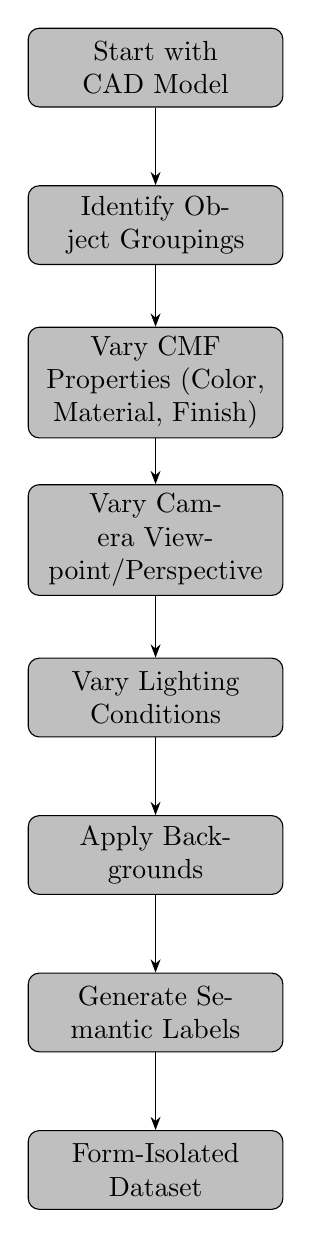
\begin{tikzpicture}[
    node distance=2cm,
    block/.style={rectangle, draw, fill=lightgray, rounded corners, minimum width=3cm, minimum height=1cm, text width=3cm, align=center},
    arrow/.style={-Stealth}
  ]

  \node[block] (start) {Start with CAD Model};
  \node[block, below of=start] (objectgrouping) {Identify Object Groupings};
  \node[block, below of=objectgrouping] (cmfvariation) {Vary CMF Properties (Color, Material, Finish)};
  \node[block, below of=cmfvariation] (cameraviewpoint) {Vary Camera Viewpoint/Perspective};
  \node[block, below of=cameraviewpoint] (lighting) {Vary Lighting Conditions};
  \node[block, below of=lighting] (background) {Apply Backgrounds};
  \node[block, below of=background] (semanticlabeling) {Generate Semantic Labels};
  \node[block, below of=semanticlabeling] (dataset) {Form-Isolated Dataset};

  \draw[arrow] (start) -- (objectgrouping);
  \draw[arrow] (objectgrouping) -- (cmfvariation);
  \draw[arrow] (cmfvariation) -- (cameraviewpoint);
  \draw[arrow] (cameraviewpoint) -- (lighting);
  \draw[arrow] (lighting) -- (background);
  \draw[arrow] (background) -- (semanticlabeling);
  \draw[arrow] (semanticlabeling) -- (dataset);

\end{tikzpicture}

\subsection{Object Grouping in CAD Models}

The system is designed to be compatible with a range of industry-standard CAD software, enhancing its accessibility and integration into existing design workflows. While the principles of the invention apply broadly, specific implementations may leverage particular features of different CAD packages. The following describes the supported software and their relevance to the invention:

\textbf{Supported CAD Software:} The system is designed for compatibility with CAD software packages that allow for hierarchical object organization and programmatic access to model data. These features are crucial for automating the variation generation and semantic labeling processes. Specifically, the current implementation supports:

\begin{itemize}
    \item \textbf{Rhinoceros 3D (Rhino):} Rhino is a powerful 3D design environment with a robust scripting API. It is discussed extensively herein because of its robust scripting capabilities using Python, allowing for deep integration with the Automated Data Generation Module. The provided Rhino and Python code show examples of this integration, which skilled practitioners can extrapolate to other design software programs and their respective APIs. 
    \item \textbf{Fusion 360:} Fusion 360, with its extensive use in engineering and product design, is also a target platform for this invention. Its Python API enables similar functionalities as in Rhino, allowing for seamless integration with the Automated Data Generation Module.
    \item \textbf{SolidWorks:} SolidWorks, another widely used CAD software, can also be integrated with the system. Its API, while primarily supporting a variant of C++, can be accessed through COM interop from Python, enabling similar functionalities as in Rhino and Fusion 360. Alternatively, the codebase providing the Automated Rendering Module could be refactored to implement the functionality natively.
\end{itemize}

Any CAD software offering similar functionalities in terms of object hierarchy and programmatic access can be integrated with the system. The core principles of the invention remain applicable across different CAD platforms. For example:


\begin{itemize}
    \item \textbf{Layers (Rhino):} In Rhino, layers provide a primary means of organizing objects. The provided code explicitly uses layers (specifically sublayers denoted by "::") to group different parts of the chair model (e.g., "Chair::Legs," "Chair::Seat," "Chair::Backrest"). This layer-based organization directly corresponds to the concept of object groupings in this invention. The code demonstrates how materials are applied to objects based on their layer assignment, highlighting the importance of this hierarchical structure for generating variations.
    \item \textbf{Components (Fusion 360):} Fusion 360 utilizes components as a fundamental organizational structure. Similar to layers in Rhino, components can represent distinct parts or sub-assemblies within a design. The system can be adapted to utilize component information for object grouping and variation generation in Fusion 360.
    \item \textbf{Groups/Bodies (SolidWorks):} SolidWorks employs groups and bodies for organizing geometry. The system can be implemented to recognize these groupings and utilize them for applying variations and generating semantic labels.
\end{itemize}

\begin{figure}[!htbp]
    \centering
    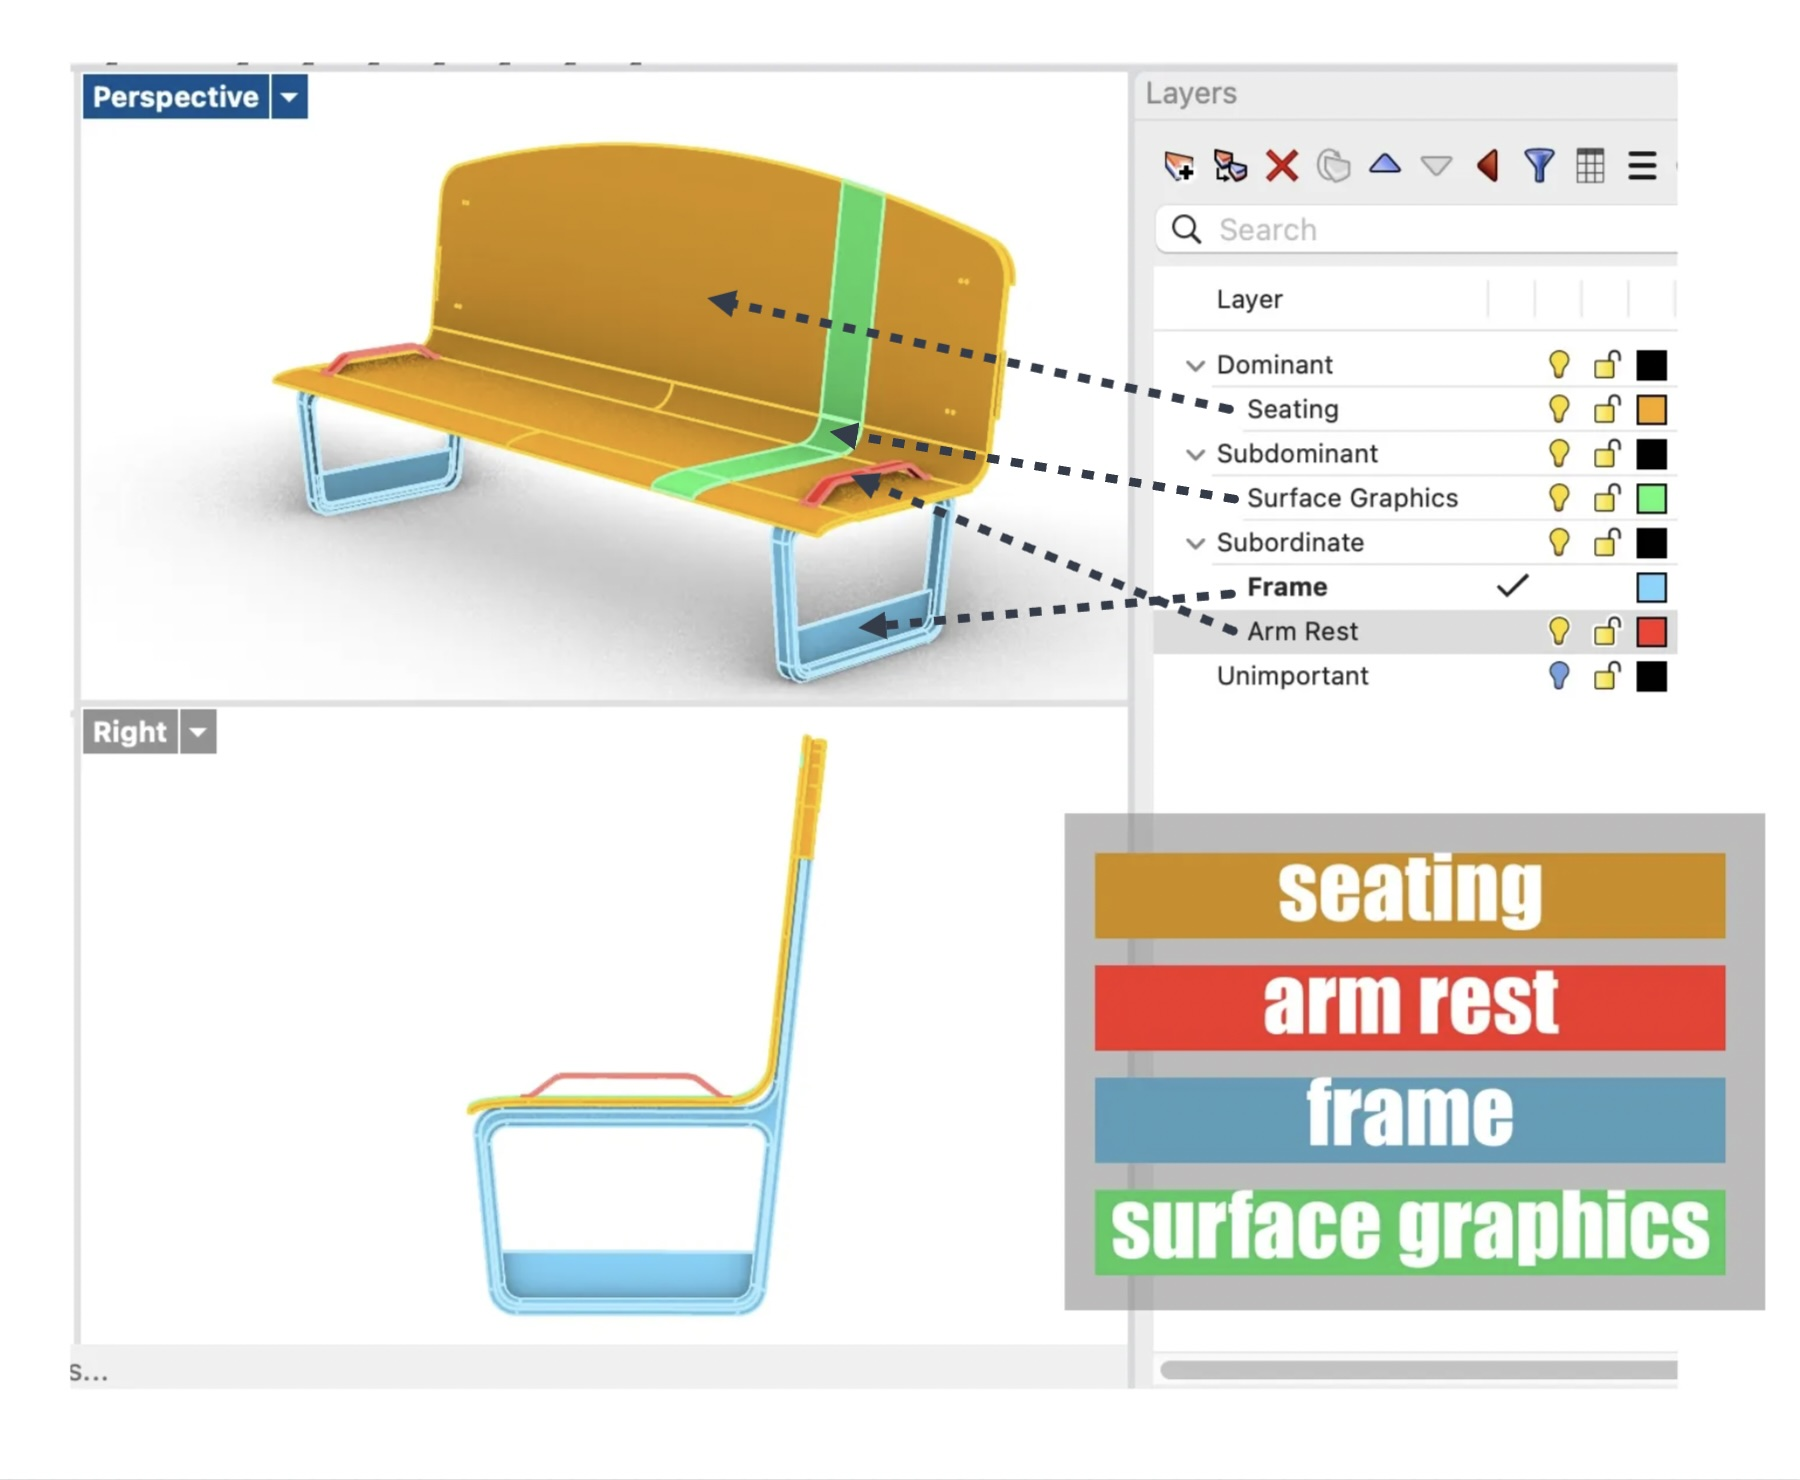
\includegraphics[width=\textwidth]{figures/figure-perspective-right-layers-colors-labled-arrows-2.jpg}
    \caption{CAD Model with Object Groupings and Layer Correspondence}
    \label{fig:cad_model_groupings}
\end{figure}

The system is designed to be adaptable to different object grouping mechanisms. The core concept of organizing objects hierarchically to represent design intent remains consistent, regardless of the specific CAD software or its internal representation of groups.

\paragraph{Importing and Preprocessing CAD Data}
The process of importing CAD models into the system and any necessary preprocessing steps are crucial for ensuring compatibility and efficient data handling.

In some cases, it may be necessary to convert the CAD geometry into a mesh representation for efficient rendering and processing. This conversion can be performed within the CAD software itself or using external libraries. The system handles mesh data appropriately, maintaining the object groupings and applying variations to the mesh elements. If mesh conversion is required, the system will ideally use the highest fidelity mesh representation available, balancing detail with computational efficiency.

For very complex CAD models, geometry simplification techniques may be employed to reduce the computational load during variation generation and rendering. Simplification techniques, such as mesh decimation or NURBS curve reduction, can be applied while preserving the overall form and object groupings. The system incorporates parameters to control the level of simplification, allowing designers to balance detail with performance. The decision to simplify geometry is context-dependent and depends on the complexity of the model and the computational resources available. The system provides feedback to the designer if simplification is necessary and allows them to adjust the simplification parameters as needed.

\subsection{Automated Data Generation Module}

The Automated Data Generation Module is the core of the invention, responsible for creating the diverse and richly labeled dataset required to train the AI model. It interacts directly with the CAD system, extracting object groupings, applying systematic variations, and generating corresponding semantic labels.

\subparagraph{Identifying Object Groupings:} This module parses the CAD model to identify object groupings based on user-defined criteria within the hierarchical organization enforced within the CAD system. The module can be considered both the Rhino template that enforces three levels of hierarchy (dominant, subdominant and subordinate) and the computer code that traverses the layers and sublayers to manipulate the objects found therein as well as return a semantic label based on chosen naming schemas of the designer.

For example, in one exemplary  CAD systes, Rhino, might see code such as the following: 

    \begin{verbatim}
        def get_objects_from_sublayers():
        """Get all objects from sublayers, organized by sublayer name."""
        sublayers = get_all_sublayers()
        objects_by_sublayer = {}
        for sublayer in sublayers:
            objects = rs.ObjectsByLayer(sublayer)
            if objects:
                objects_by_sublayer[sublayer] = objects
        return objects_by_sublayer
    \end{verbatim}  

This explicit modularity, provided as layer-based grouping in Rhino (as an example), provides a direct mapping between the CAD model's organization and the system's understanding of design components.


\subsection{User Interface for Variation Setup and Semantic Label Generation}

\begin{figure}[h]
    \centering
    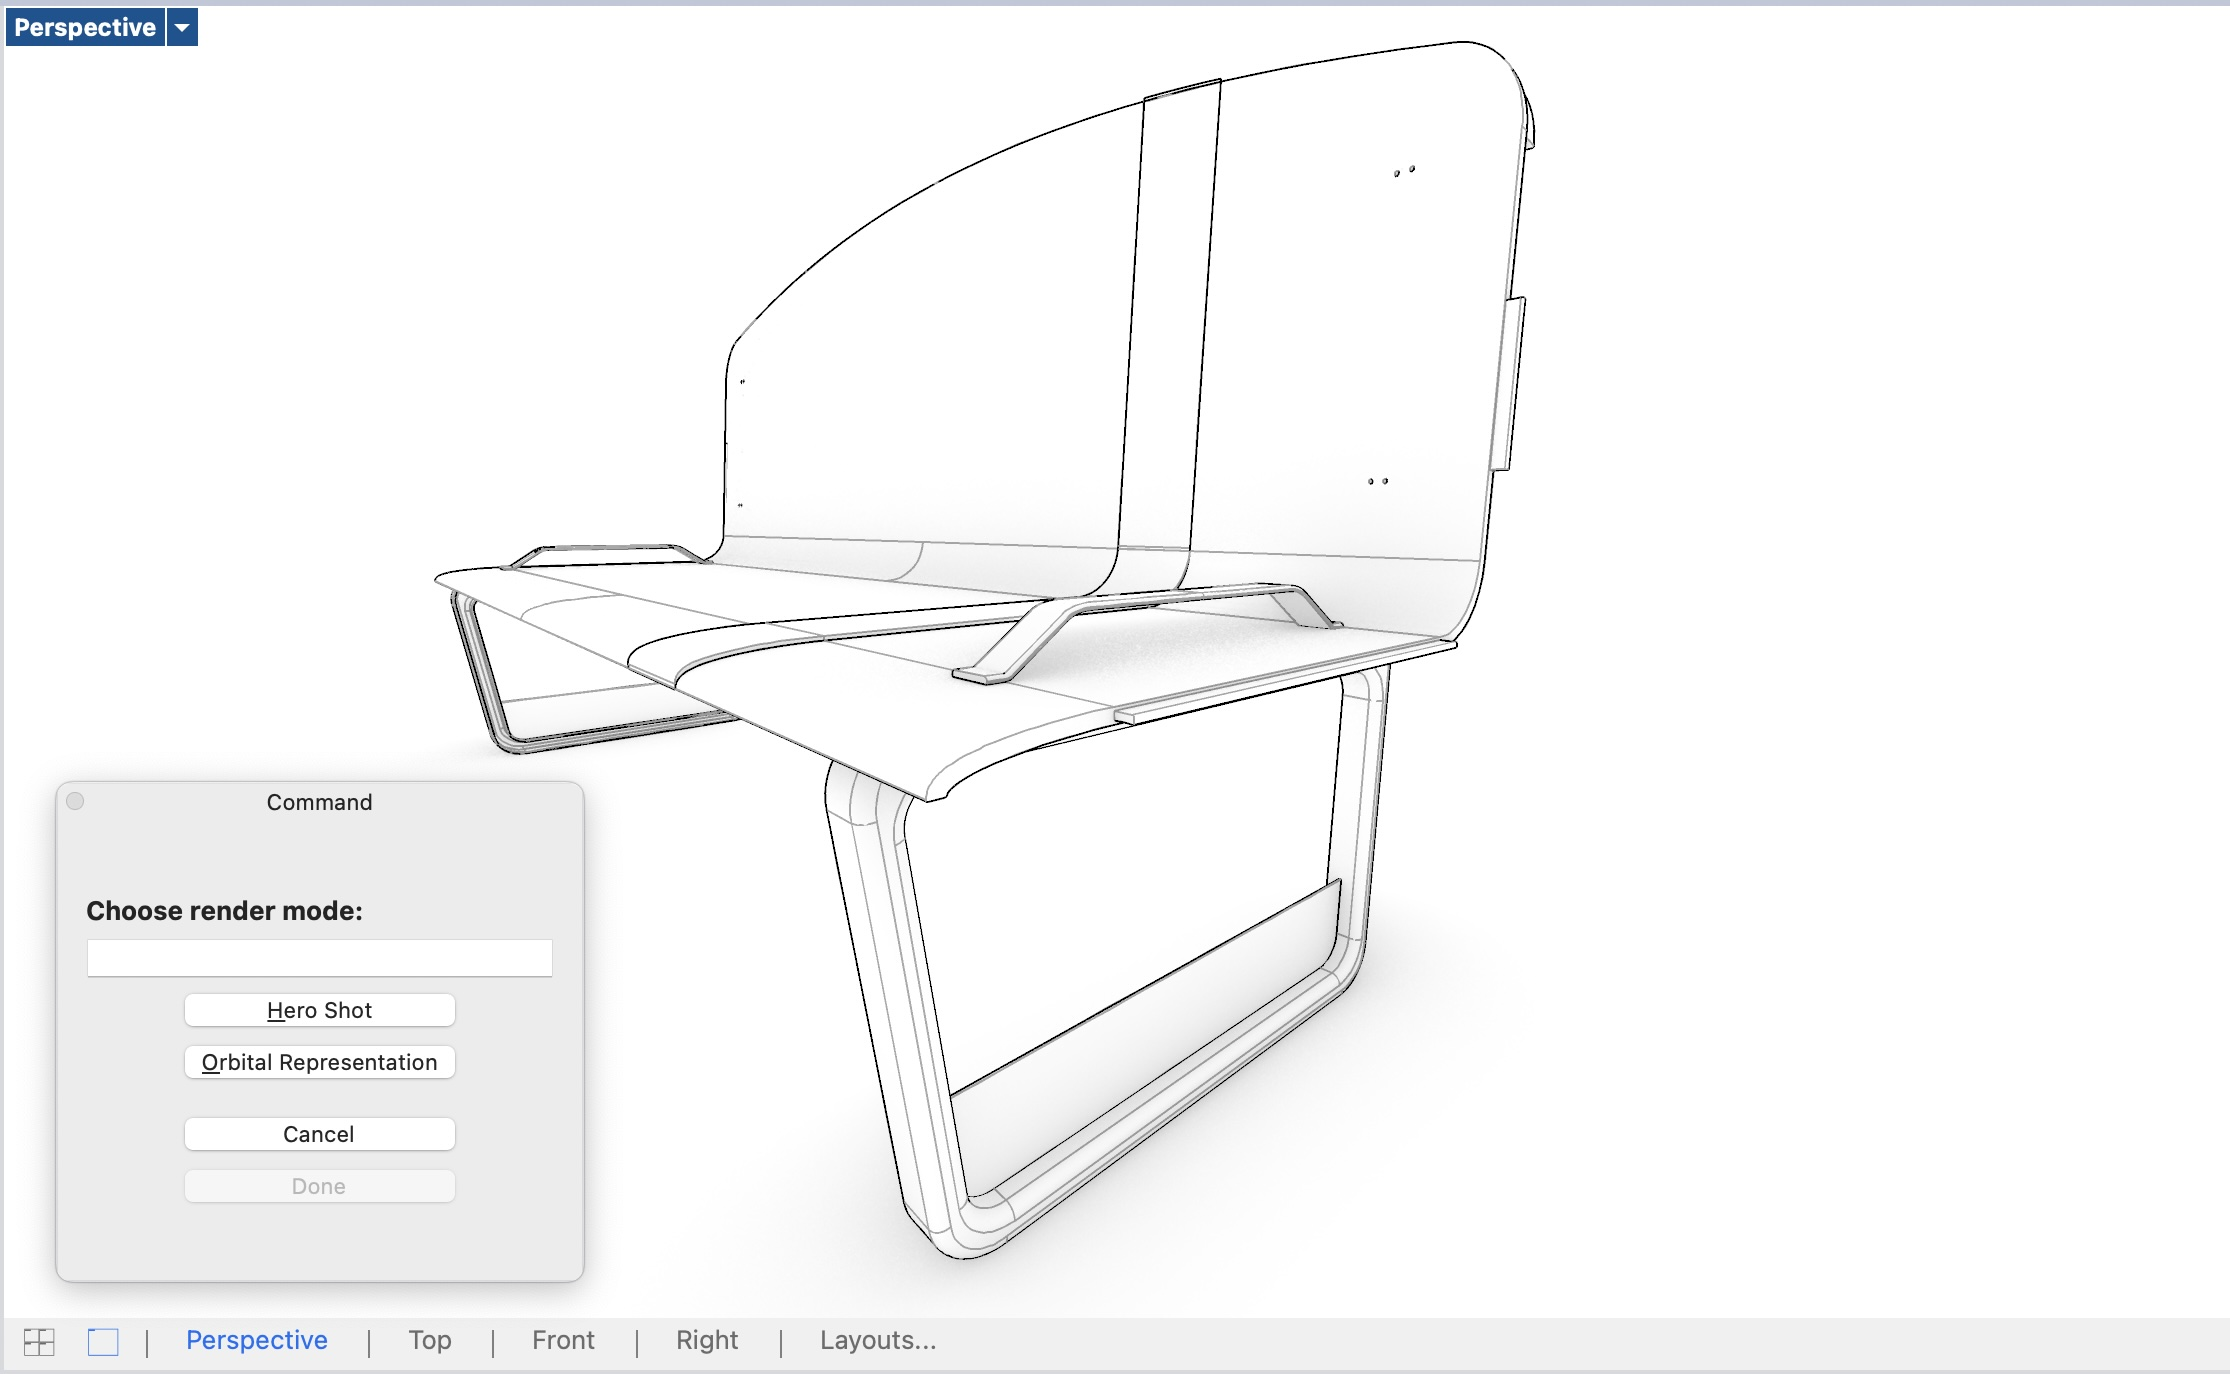
\includegraphics[width=0.8\textwidth]{figures/figure-process-choose-render-mode-monochrome.jpg} 
    %    \caption{Step \arabic{figCounter}
    \caption{Step   Selecting the Rendering Mode - The user interface allows the designer to choose between different rendering modes, such as "Hero Shot" for focused product-style renders and "Orbital Representation" for a more comprehensive 360-degree view of the design. This flexibility enables the generation of a diverse dataset capturing the object from various perspectives.}
    \label{fig:render_mode_selection_unique}

\end{figure}

\begin{figure}[h]
    \centering
    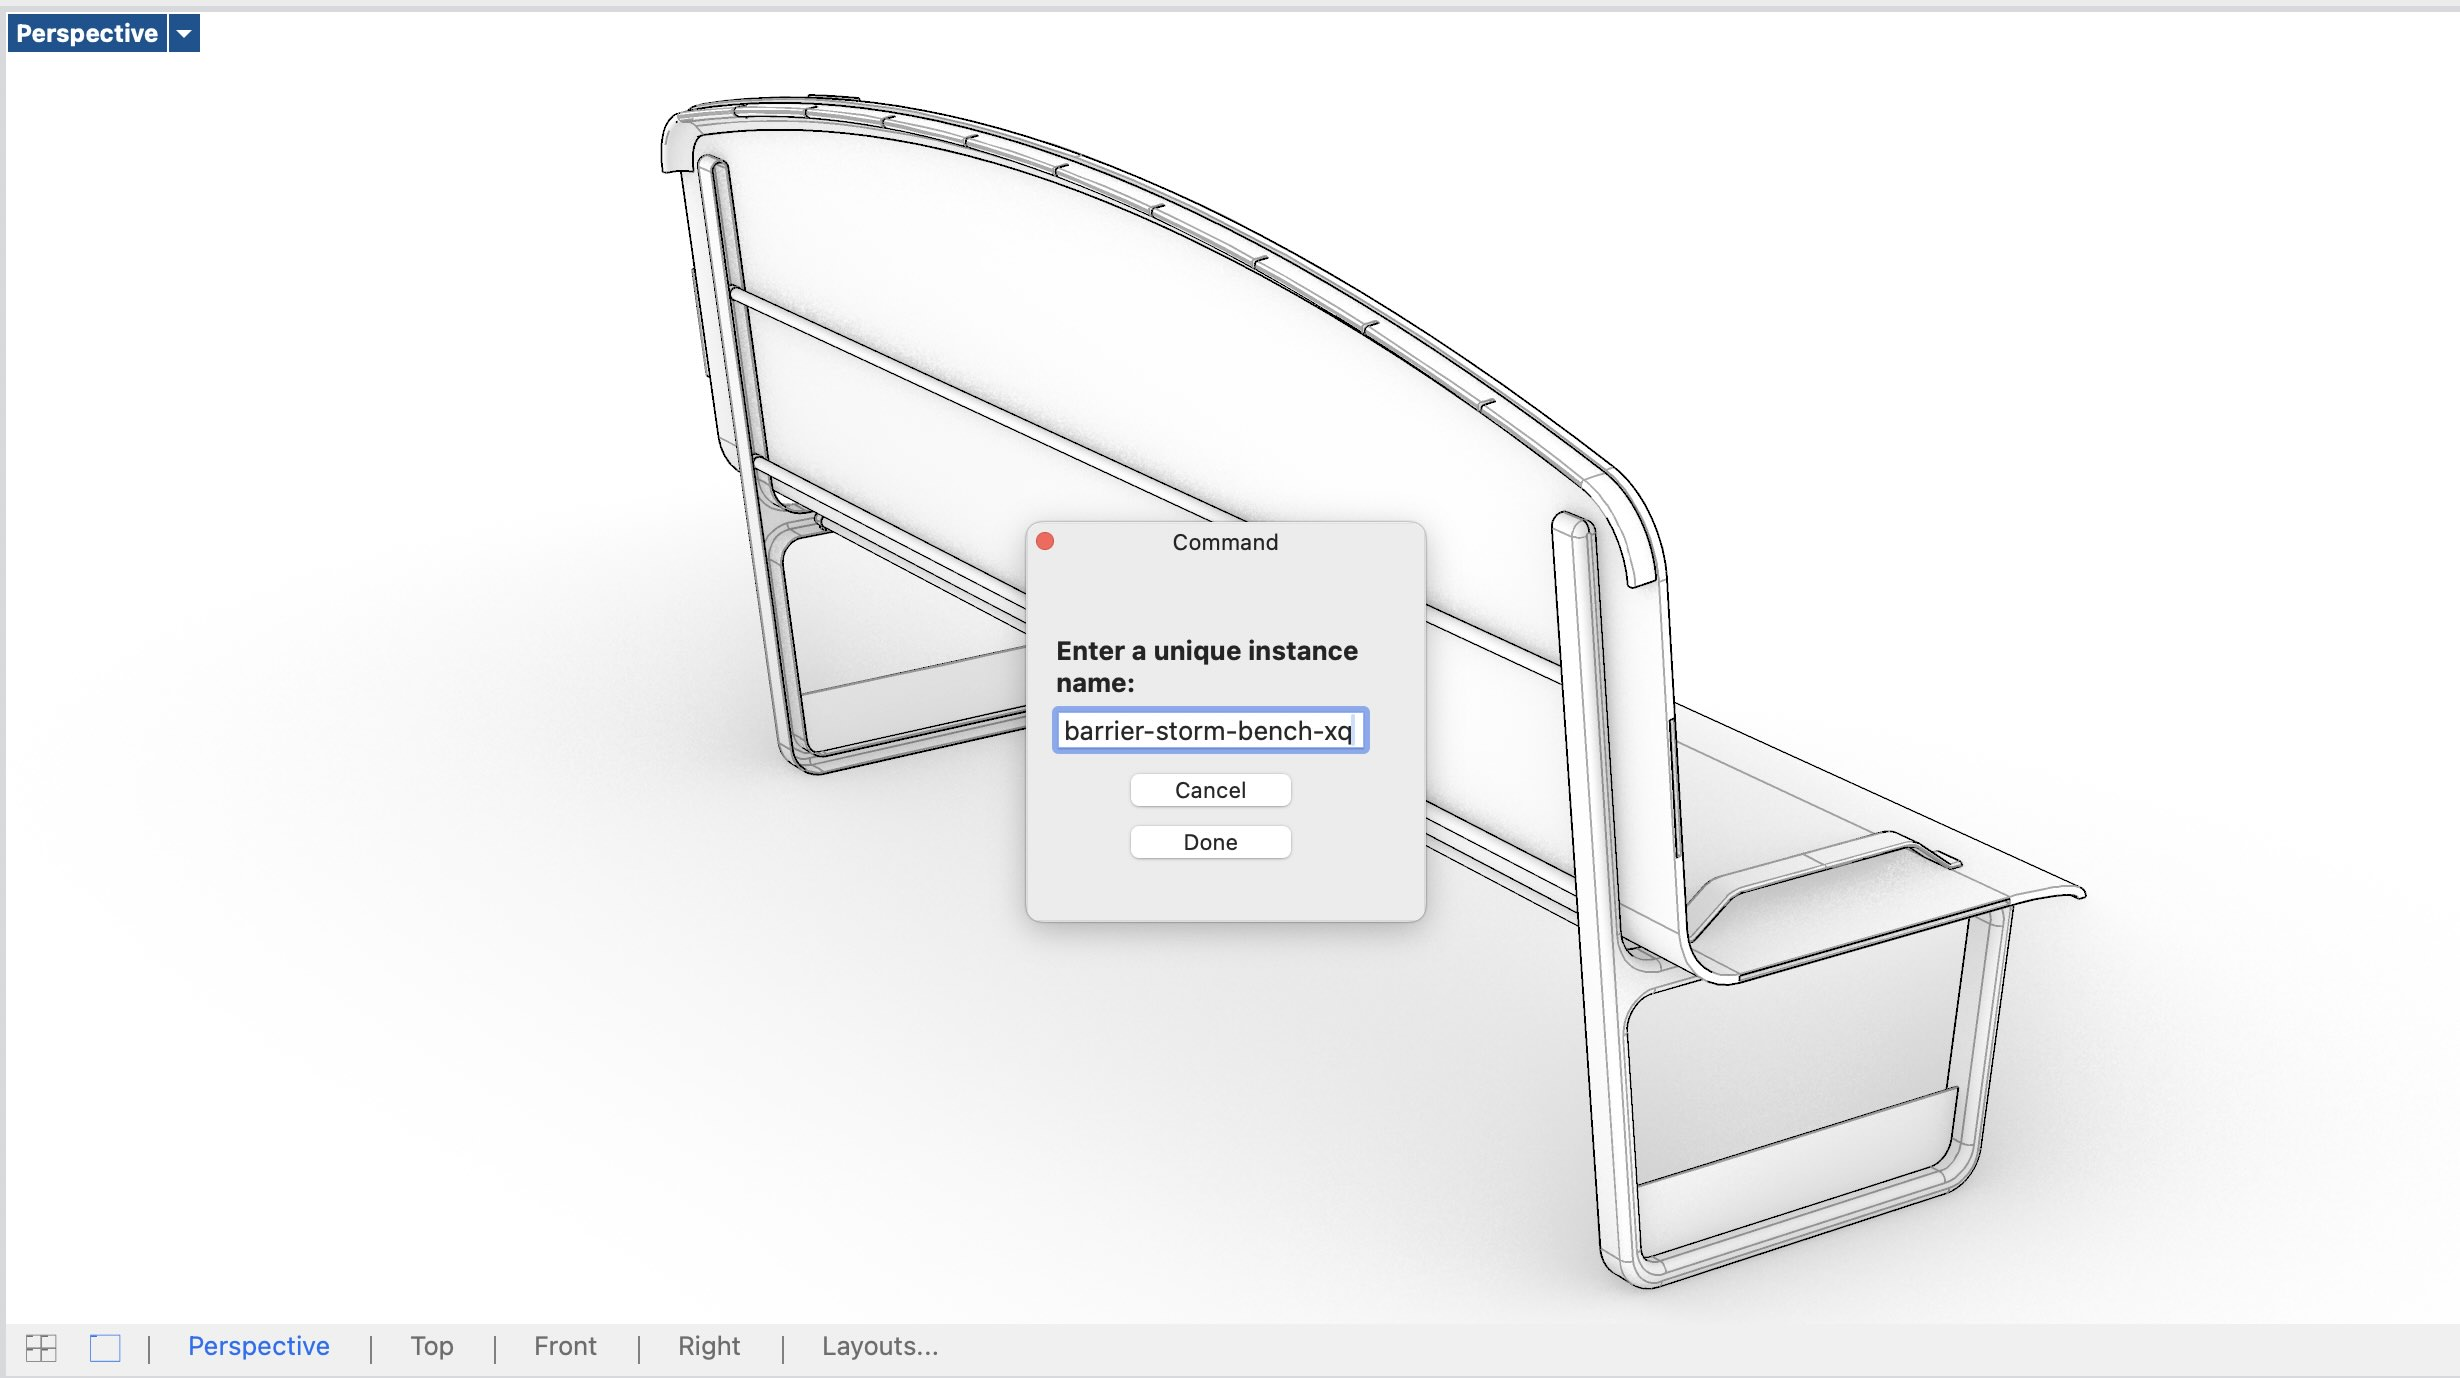
\includegraphics[width=0.8\textwidth]{figures/figure-process-instance-name-barrier-1up-xy-monochrome.jpg}
    \caption{Entering a Unique Instance Name - The user interface prompts the designer to enter a unique instance name for the object being rendered. This instance name, along with other relevant information (class name, lighting, etc.), forms part of the semantic label for each generated variation. These labels provide textual descriptions that help the AI model associate visual features with specific attributes.}
    \label{fig:instance_name_input}
\end{figure}

\begin{figure}[h]
    \centering
    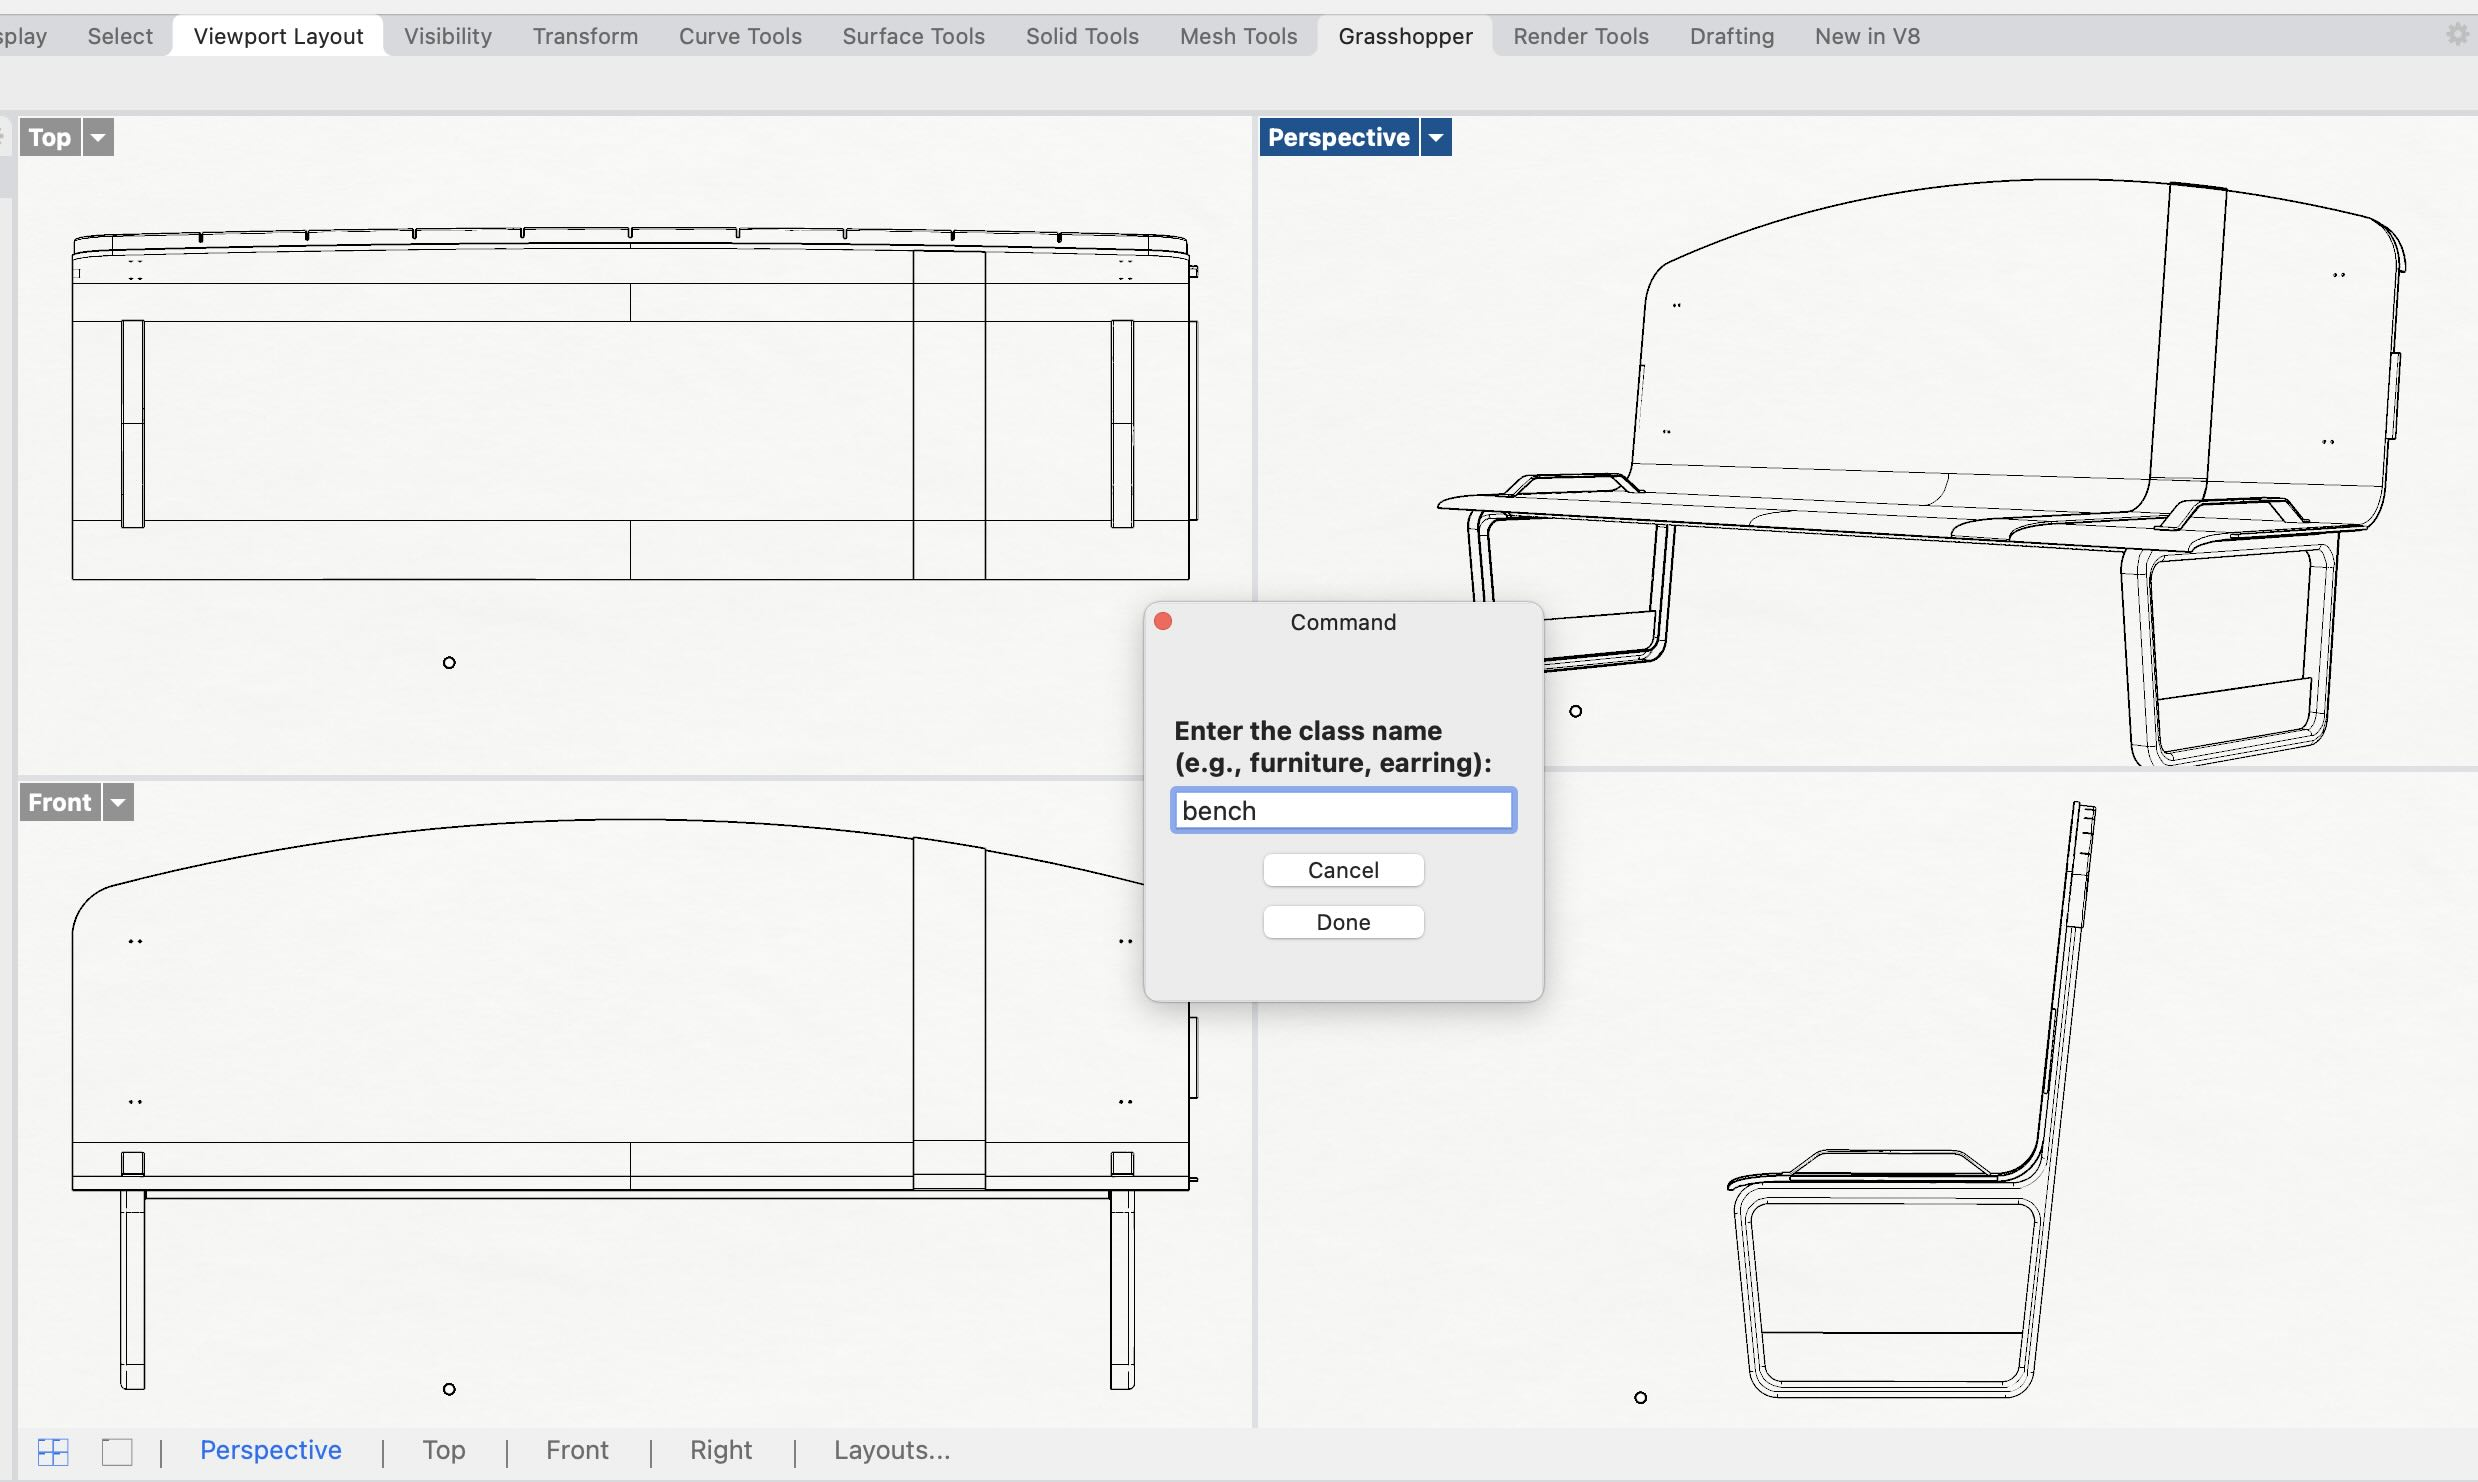
\includegraphics[width=0.8\textwidth]{figures/figure-process-class-name-bench-4up-bw.jpg}
    \caption{Specifying the Class Name - The user interface prompts the designer to enter a class name for the object, providing a broader categorization that helps the AI model understand the object's general type (e.g., furniture, vehicle, appliance). This class name, along with the instance name and other details, forms part of the semantic label for each variation.}
    \label{fig:class_name_input}
\end{figure}

\begin{figure}[h]
    \centering
    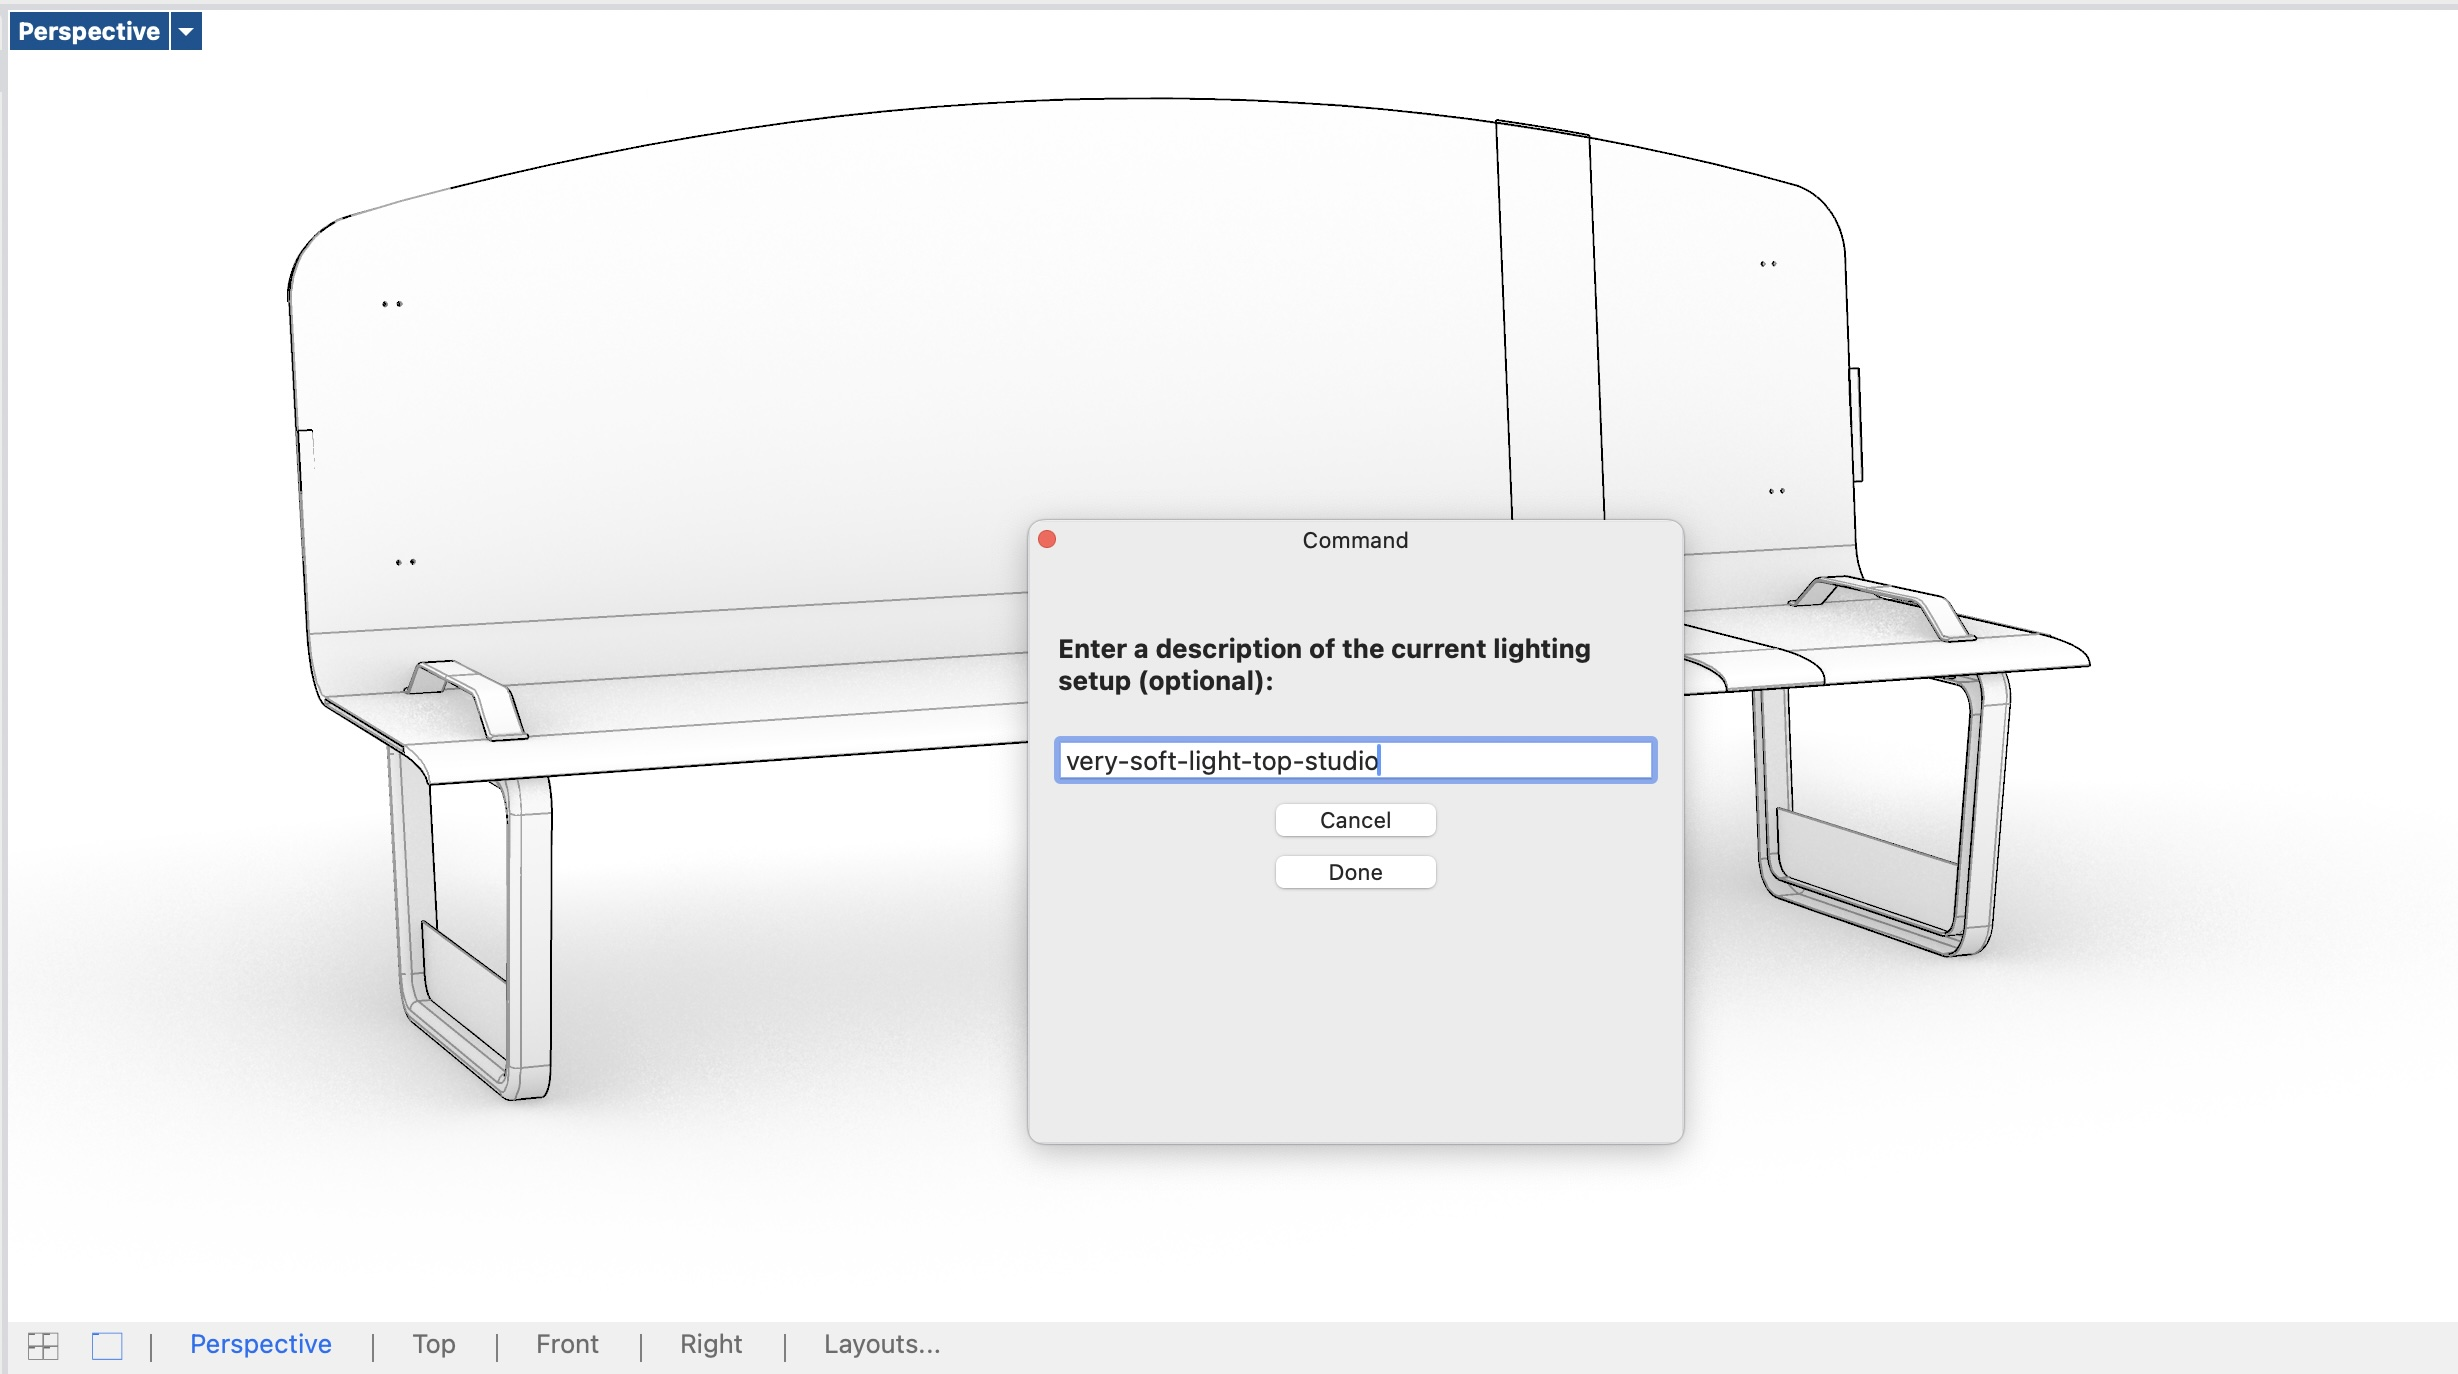
\includegraphics[width=0.8\textwidth]{figures/figure-process-light-description-monochrome.jpg}
    \caption{Describing the Lighting Setup - The user interface allows the designer to enter a description of the lighting setup used for each rendering. This information, captured as part of the semantic label, enables the AI model to learn the relationship between lighting conditions and the object's appearance. In this example, the description "very-soft-light-top-studio" provides a concise representation of the lighting setup.}
    \label{fig:lighting_description_input}
\end{figure}


\subsection{Generating Variations:} This module systematically applies variations to the CAD model across four key aspects: visual properties, camera viewpoints and perspectives, lighting conditions, and backgrounds.

\subsubsection{Object Visual Properties}

\textbf{Visual Properties (CMF):} The system varies the color, material, and finish (CMF) properties of objects within the defined groupings.

\begin{figure}[h]
    \centering
    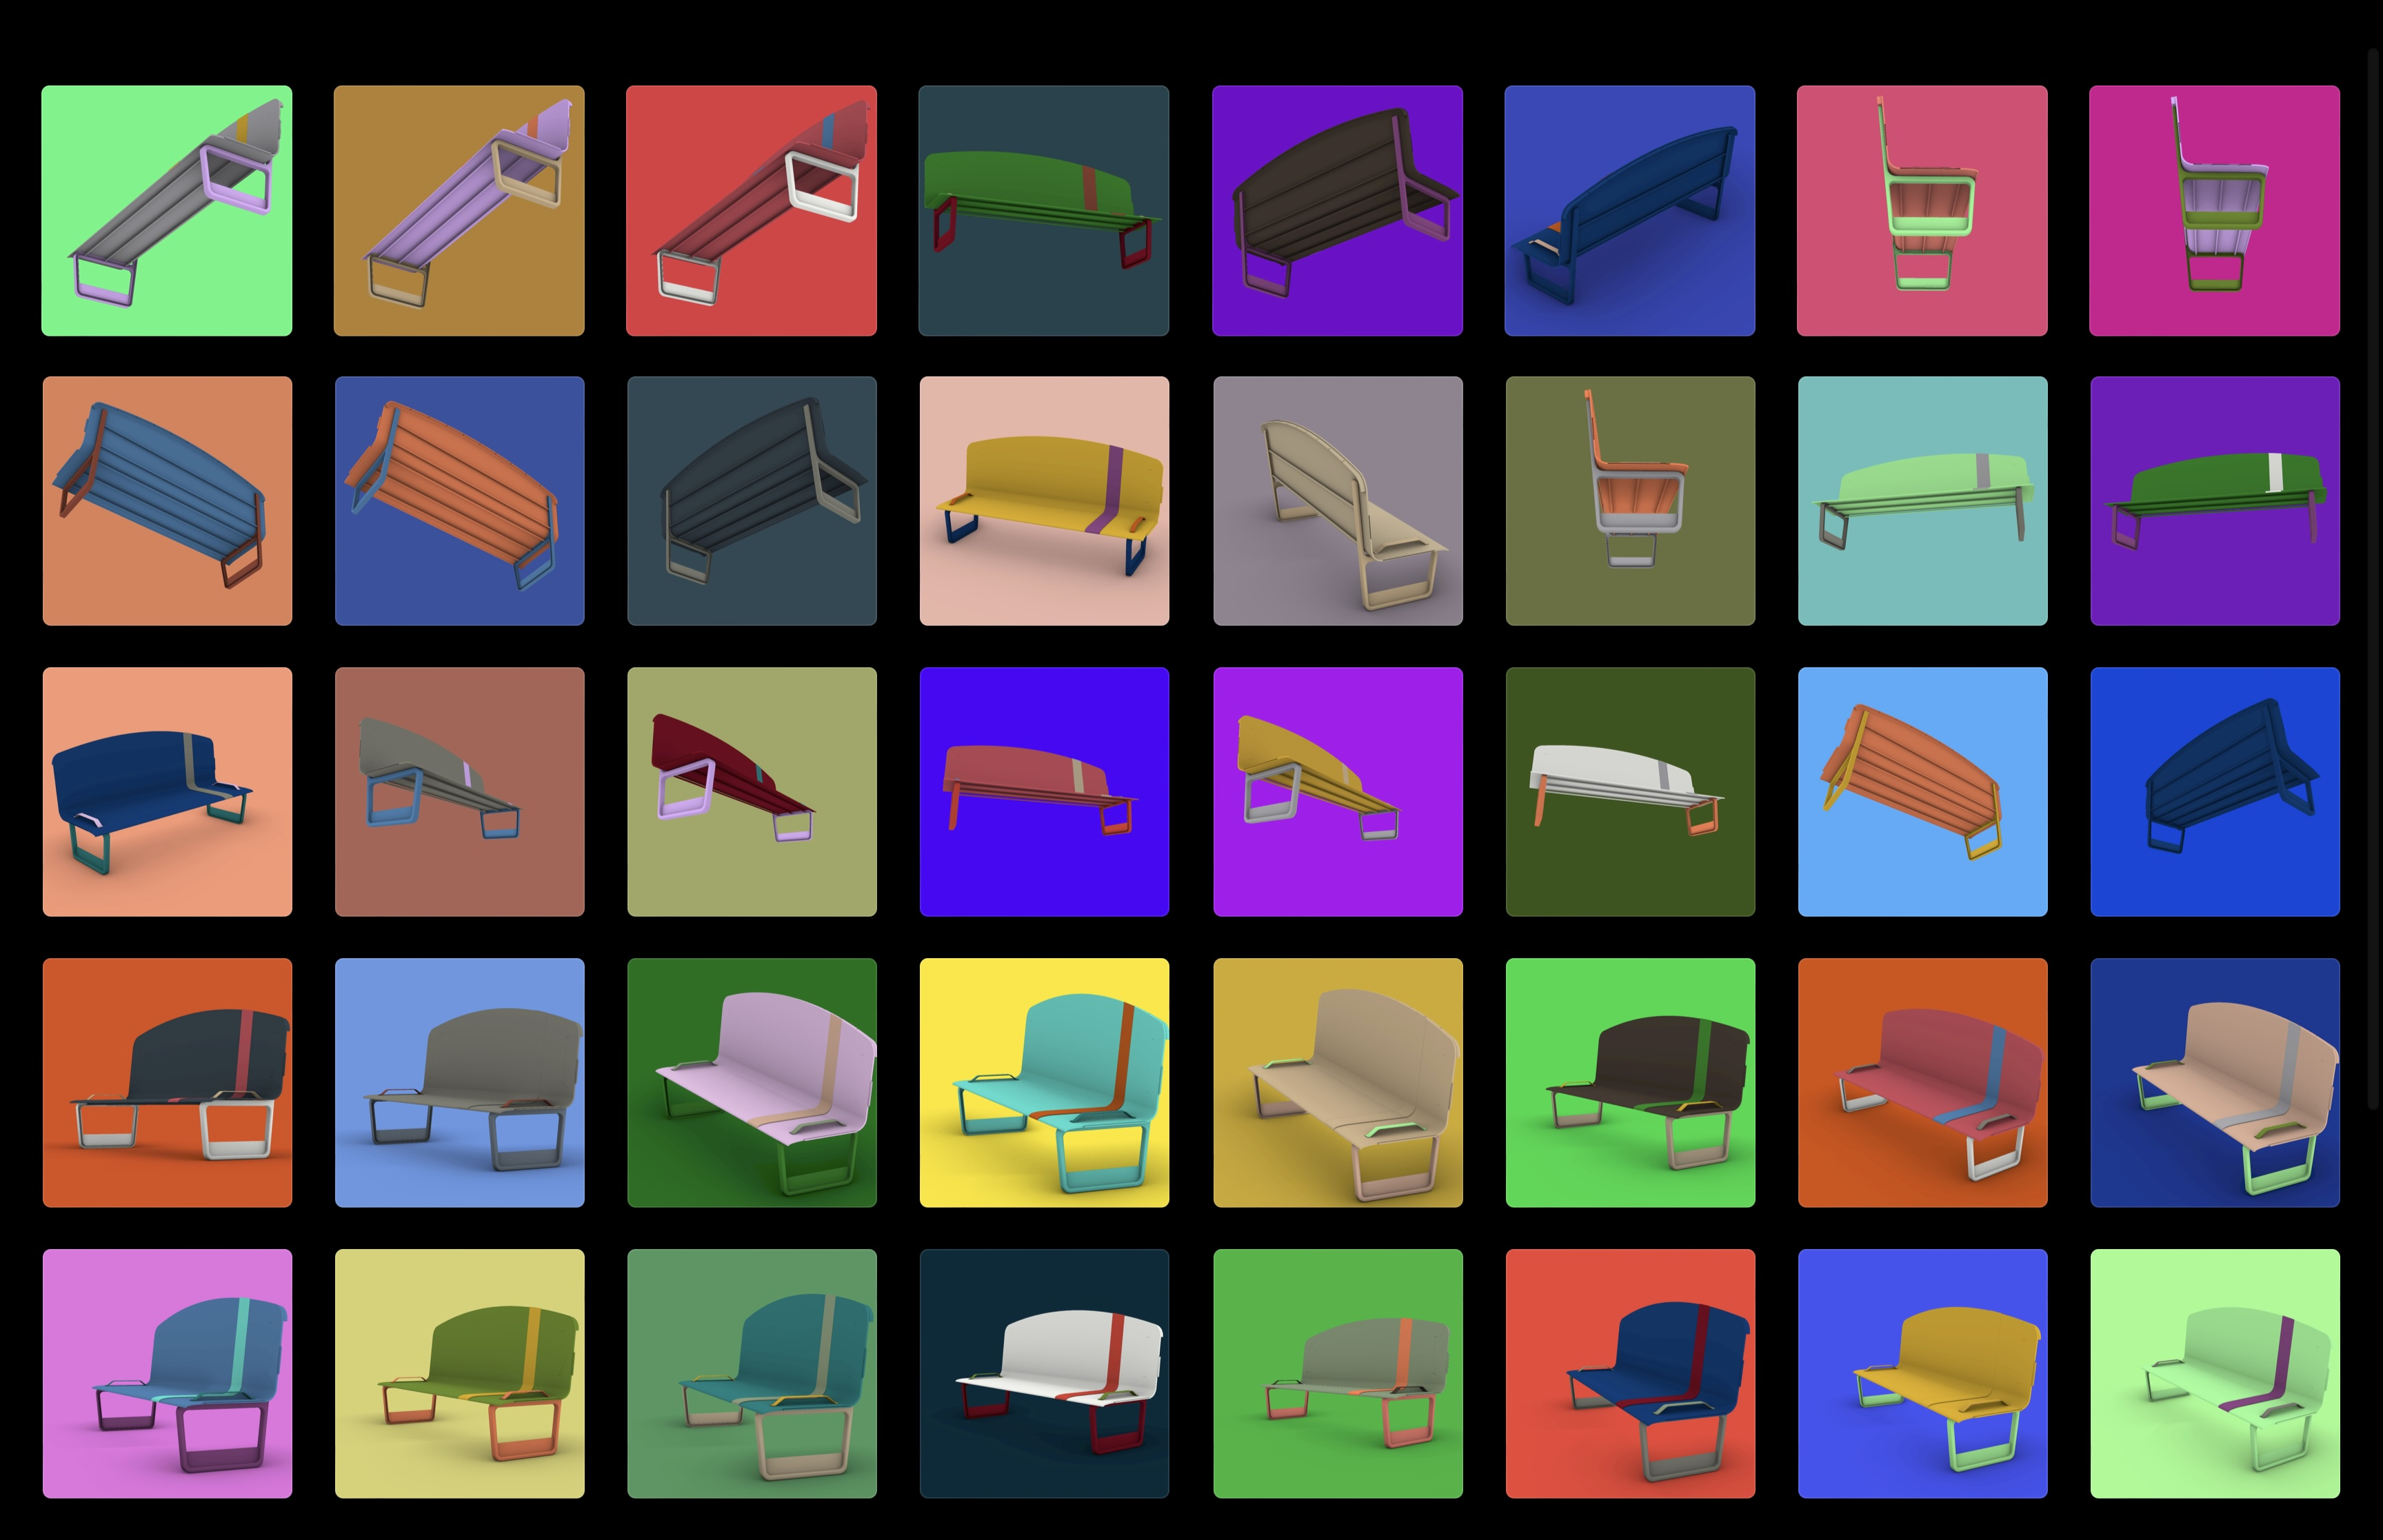
\includegraphics[width=0.8\textwidth]{figures/figure-process-orbital-and-hero-shot-combined-color.jpg} 
    \caption{The output of both 'hero mode' and product-style perspective renders and "Orbital Representation" to provide comprehensive 360-degree views of the design. The contribution of angles and emphasis isdiscussed to a diverse dataset is discussed in more detail elsewhere but is to be appreciated visually here.}
    \label{fig:render_mode_selection}
\end{figure}

\textbf{Randomness and Predefined Ranges:}

The code example showcases the use of randomness and predefined ranges for material assignment. For example, a data structure such as \texttt{MATERIAL\_LIST} defines a library of materials with their associated properties (name, RGB color, gloss, and reflectivity). A function with a name such as \texttt{create\_random\_material()} randomly selects a material from this list and applies it to the objects within a group. This randomized approach ensures a diverse range of CMF variations in the training dataset. The system also allows for user-defined ranges for each CMF property, providing more control over the variation process. For example:

        \begin{verbatim}
        
    MATERIAL_LIST = [
    ("Soft Red Plastic", (220, 60, 50), 30, 0.2),
    ("Forest Green Metal", (34, 139, 34), 80, 0.5),
    ("Navy Blue Fabric", (0, 60, 120), 20, 0.1),
    ("Mustard Yellow Leather", (225, 173, 1), 40, 0.15),
    ("Teal Ceramic", (0, 128, 128), 70, 0.2),
    ("Plum Wood", (142, 69, 133), 50, 0.3),
    ("Off White Paint", (245, 245, 240), 25, 0.1),
    ("Charcoal Rubber", (54, 69, 79), 35, 0.05),
    ...etc...
\end{verbatim}

To apply random materials to all objects in sublayers, while keeping track of of the material choices for labeling purposes, we might use code such as the following:

\begin{verbatim}

    def apply_random_materials():

    objects_by_sublayer = get_objects_from_sublayers()
    materials = {}
    
    for sublayer, objects in objects_by_sublayer.items():
        material_index, material_name = create_random_material()
        
        for obj in objects:
            rs.ObjectMaterialIndex(obj, material_index)
        
        sublayer_name = sublayer.split("::")[-1].lower()
        
        # Create a grammatically correct description
        description = f"{material_name} {sublayer_name}"
        
        materials[sublayer_name] = {
            'name': sublayer_name,
            'material': material_name,
            'description': description
        }
    
    print(f"\nApplied materials: {materials}")
    return materials
        \end{verbatim}

\subsubsection{Camera Viewpoints and Perspectives}

The system varies the camera perspective to capture the design from different angles and distances. Many ways of doing this are possible. Consider two examples as implemented in Rhino: \texttt{Hero Shot} and \texttt{Orbital Representation}. "Hero shot" generates camera positions clustered around a focal point, simulating product photography. Importantly, the primary focal point is chosen by the designer. The \texttt{'variation\_degrees'} parameter controls the degree of randomness in camera positioning within components of the automated data generation model such as 'Hero Shot'.Thus one representative sample of the object is clustered around a viewpoint representing a preferred view of the object by the designer. Because such preferred views are labled, aspects of the preferred view such as focal lentgh, azimuth, inclination, object orientation relative to groundplane and other aspects of composition (virtual or otherwise) can be trained into the AI model. "Orbital representation" generates camera positions along one or many circular, elliptical  orbits around the object, providing a more comprehensive view of the design. Designers and other parties will appreciate that the form governing or representing the path traversed by the virtual camera used in automated rendering is not limited to circles or ellipses and can be one of many patterns

The \texttt{generate\_viewpoint\_description()} function, as an example, demonstrates how variation in focal length can be implemented, simulating different lens effects and perspectives. This adds additional variation to the generated renders to avoid overfitting in training.


\subsubsection{Lighting} 

The system generates diverse lighting scenarios, mimicking different environments and times of day.

For example, a function such as \texttt{generate\_lighting\_variation()} can create and store variation in lighting softness, direction, and intensity, as well as save the parameters of the settings and their corresponding natural language description to be used during the labeling process. 


\subsubsection{Backgrounds}

The system applies different backgrounds to the rendered images, enhancing context and visual diversity.

A library of predefined backgrounds, including solid colors, gradients, textures, patterns, and environmental scenes, is used to create variations. The language required for such a background can be pulled from a CLIP inference, from a library of knowledge, from the file name itself, or from various other metadata, or a combination thereof.

Additionally, the system integrates with Google Maps, allowing designers to use real-world locations as backgrounds. This function utilizes depth maps derived from Google Maps data and ControlNet to ensure accurate placement and perspective of the 3D model within the chosen environment. 

\paragraph{Semantic Label Generation:} For each generated variation, the system creates a detailed semantic label.

\begin{itemize}
    \item \textbf{Structured Description:} The \texttt{generate\_caption()} function in the code provides a basic example of semantic label generation. The full system generates more comprehensive labels, incorporating information about:
    \begin{itemize}
        \item \textbf{Object Groupings and Materials:} "Chair legs made of brushed aluminum, seat upholstered in dark blue fabric, backrest made of light wood."
        \item \textbf{Camera Viewpoint:} "Viewed from a high angle, front right perspective, with a 50mm lens."
        \item \textbf{Lighting Conditions:} "Illuminated with soft, natural light from the left."
        \item \textbf{Background:} "Against a neutral gray background."
    \end{itemize}
\end{itemize}

The detailed semantic label can be utilized in the generation of the file name for the specific image rendered, or concatenated with other labels into a JSON file or other data structure sufficient to describe each of the images used in fine-tuning the generative AI model. 

This structured approach ensures consistency and facilitates the AI model's understanding of the relationship between textual descriptions and visual attributes.

\subparagraph{Synthetic Augmentation Techniques:} To maximize the diversity of the training dataset and improve the AI model's robustness, the system may utilize various data augmentation techniques, for example:

\begin{itemize}
    \item \textbf{Random Cropping:} Randomly cropping sections of the rendered images.
    \item \textbf{Rotation and Flipping:} Rotating and flipping components to create variations in orientation. It is to be appreciated that because they are flipped in their CAD enviorment as opposed to merely rotating the automatically rendered image, any simulated interaction between the form and its enviorment may be shown. For example, flipping an element in Maya relative to the gravity vector in Maya will cause elements created with nCloth, a flexible mesh simulation, to fall along the gravity vector. In such a way, the essential properties of the form in addition to the form may be deeply encoded into the model by means in addition to mere semantic labeling. One should note that rotation of images may still be done to enrich the training set, but such rotation is properly labled. It is to be appreciated that specialty language used by cinematographers and photographers, such as "dutch angle" may be utilized in a virtual camera enviorment to aptly label the variation to the outputted image. 
    \item \textbf{Color Jitter:} Randomly adjusting brightness, contrast, saturation, and hue.
    \item \textbf{Noise Addition:} Adding small amounts of random noise to the images to simulate real-world imperfections.
\end{itemize}

These techniques artificially expand the training dataset, improving the AI model's ability to generalize and reducing the risk of overfitting. The specific data augmentation techniques used can be customized and adjusted based on the design context and the characteristics of the dataset.

\subsubsection{Summary}

In summary, the systematic variation of visual properties, camera viewpoints, lighting conditions, and backgrounds, combined with the automated generation of semantic labels, forms the foundation for training a robust and versatile AI model for design applications. The referenced code examples illustrate how these functionalities are implemented in practice, demonstrating the practicality and effectiveness of the invention.

\subsection{AI Model Training Module}

This module is responsible for imbuing the AI with the ability to understand and generate variations of the designer's intended form. Instead of merely learning to associate specific visual styles with a design, the AI is trained to recognize and reproduce the form itself as the primary element, independent of potentially distracting variations in color, material, texture, lighting, or viewpoint. This is achieved by leveraging the meticulously curated dataset generated by the Automated Data Generation Module, which embodies the core principle of form isolation.

\subsubsection{Pre-trained Model Selection}
The system starts with a pre-trained text-to-image AI model, chosen from a range of suitable options. Key criteria for model selection could include:

\begin{itemize}
    \item \textbf{Open-Source License:} Essential for maintaining complete ownership and control over the technology, allowing for unrestricted customization, private deployment, and future development.
    \item \textbf{Architectural Flexibility:} The model's architecture should be adaptable for fine-tuning, ideally through efficient techniques like Low-Rank Adaptation (LoRA), which allow for targeted modification without retraining the entire model.
    \item \textbf{Adequate Image Quality:} The model should be capable of generating images with sufficient quality and resolution for design visualization purposes. However, perfect photorealism is not necessarily the primary goal at this stage; the focus is on the model's ability to learn and represent form.
\end{itemize}

Examples of potential open-source models include Stable Diffusion or other emerging diffusion-based models known for their flexibility and efficiency. The specific choice of model is not critical to the invention; rather, it's the subsequent training process that imbues the model with the unique capability to understand and generate design forms independently of stylistic variations.

\subsubsection{Training for Form Recognition}
Unlike conventional approaches that focus on teaching the AI to mimic specific visual styles or aesthetics, this system trains the AI to recognize and reproduce the underlying form of the design as the primary element. This is achieved by leveraging the unique dataset generated by the Automated Data Generation Module.

\paragraph{Dataset Structure:} The dataset consists of numerous variations of the same design, where the form remains constant while all other visual attributes (CMF properties, camera viewpoints, lighting, backgrounds) are systematically and randomly varied. This forces the AI to focus on the only consistent element across all images: the form itself.

\paragraph{Semantic Label Guidance:} The semantic labels accompanying each image reinforce this focus on form. Instead of merely describing the specific visual features present in each image, the labels emphasize the underlying form and its constituent parts. For example, a label might read: "A chair with [varied material] legs, a [varied material] seat, and a [varied material] backrest, viewed from a [varied angle]." This structured labeling, combined with the dataset's visual emphasis on form, guides the AI to learn a representation of the form that is decoupled from specific stylistic choices.

\subsubsection{Fine-tuning with LoRA}
Low-Rank Adaptation (LoRA) is a highly efficient fine-tuning technique that allows the pre-trained model to learn from the custom dataset without retraining the entire model from scratch. 


This is particularly beneficial when working with large, complex models:

\begin{itemize}
    \item \textbf{Targeted Modification:} LoRA injects small, low-rank matrices into specific layers of the pre-trained model, allowing for targeted modifications that specialize the model's behavior without disrupting its general capabilities. This ensures that the model retains its ability to understand and generate images from text prompts while also incorporating the unique knowledge gained from the form-focused dataset.
    \item \textbf{Preventing Overfitting:} LoRA's efficiency is particularly valuable in this context. Because the training dataset consists of numerous variations of the same form, there is a risk of the model overfitting to the specific variations present in the dataset. LoRA's ability to adapt the model with minimal parameter changes mitigates this risk, ensuring that the model learns the general concept of the form rather than memorizing the specific variations seen during training.
\end{itemize}

In addition, multiple LoRAs may be used in combination on the same foundational model, allowing designers to create renders of two or more unique previously unknown (to the model) objects simultaneously within the same scene. For example, a new design for a chair could be rendered alongside a new design for a table. Because fine-tuning is performed using LoRAs, the designer could select both of those forms to be actively available in the interface and then specify that the table is on the chair, or that there are three chairs clustered around the table. 

\subsubsection{Evaluation and Validation}
The training process is closely monitored and evaluated to ensure that the model is effectively learning to recognize and generate the intended form.

\begin{itemize}
    \item \textbf{Visual Inspection:} Designers play a crucial role in evaluating the model's outputs. They visually inspect the generated images to assess their fidelity to the original form, ensuring that the AI is capturing the essential design elements and relationships.
    \item \textbf{Quantitative Metrics:} Objective metrics like Fréchet Inception Distance (FID) and CLIP Score could be used to measure the quality and relevance of the generated images. However, these metrics are interpreted in the context of the invention's specific goal: The focus is not solely on generating photorealistic images but rather on ensuring that the generated images accurately represent the intended form, regardless of the stylistic variations applied.
    \item \textbf{Generalization Tests:} The model is tested on unseen prompts and variations to assess its ability to generalize beyond the specific examples seen during training. This ensures that the AI can effectively generate novel variations of the form, responding to designer prompts that specify new CMF properties, lighting conditions, or viewpoints while still preserving the essential design characteristics.
\end{itemize}

\subsubsection{Summary}
The form-isolated dataset, combined with targeted fine-tuning using LoRA, enables the AI to learn and generalize the designer's intended form as the primary element, decoupling it from specific stylistic variations. This approach is central to the invention's ability to empower designers with unprecedented control over visual attributes while maintaining the integrity of their original design.

\subsection{AI-Assisted Design Interface}

This component serves as the bridge between the designer's intent and the AI's rendering capabilities. It's a user-friendly interface that empowers designers to interact with the trained AI model through natural language, leveraging its unique ability to generate variations of a design while preserving its core form. The interface goes beyond basic text-to-image functionality, incorporating a suite of advanced features designed to streamline the design workflow, enhance creative exploration, and facilitate collaboration.

\subsubsection{Core Rendering Functionality}

\textbf{Natural Language Prompts}: Designers interact with the AI using natural language descriptions. They can specify desired changes to the CMF properties of the design, adjust lighting conditions, request specific camera viewpoints, and even incorporate elements like characters or backgrounds. 

\textbf{Prompt Parsing and Parameter Translation}: The interface parses the designer's text prompt, identifying key elements and translating them into rendering parameters that the AI model can understand. It looks for agreement between the word choices used in the prompt and the words used to describe the model in the training process, evoking key unique trigger words when necessary if not explicitly evoked. This involves natural language processing techniques to extract relevant information from the prompt, such as:

\begin{itemize}
\item \textbf{Object References}: Identifying which parts of the design the prompt refers to (e.g., "the legs," "the seat," "the backrest"). This leverages the object groupings defined in the CAD model.
\item \textbf{CMF Properties}: Extracting desired changes to color, material, and finish. For example, "make the legs brushed aluminum," "upholster the seat in blue fabric," or "give the backrest a wood grain texture."
\item \textbf{Lighting and Viewpoint}: Interpreting descriptions of lighting conditions (e.g., "soft natural light," "dramatic spotlight") and camera viewpoints (e.g., "front view," "isometric perspective").
\end{itemize}

\textbf{Rendering Generation}: The AI model, guided by the extracted parameters, generates a rendering of the design, incorporating the specified changes while preserving the integrity of the original form. The model's ability to separate form from style, as trained by the form-isolated dataset, is crucial here. It allows designers to freely manipulate visual attributes without altering the fundamental design.

\subsubsection{Advanced Features}

In addition to the fundamental rendering capabilities, the interface provides an extensive array of sophisticated features designed to optimize and streamline the design workflow:

\subsubsection{Automated File Management}
\begin{itemize}
\item \textbf{Automated Naming}: The system generates descriptive file names for renderings based on the prompt content, eliminating manual naming and ensuring easy identification. For example, a prompt like "chair with red fabric seat, side view, warm lighting" might result in a file name like \textit{Chair\_RedFabricSeat\_SideView\_WarmLighting.jpg}.
\item \textbf{Cloud Storage}: Renderings and associated data can be automatically stored in the cloud, providing secure access from anywhere and facilitating collaboration. Version control is integrated, allowing designers to track changes and revert to previous versions if needed.
\item \textbf{Archiving}: Projects and related data can be archived for future reference, ensuring easy retrieval and organization.
\end{itemize}

\subsubsection{Detailed Close-Ups}
\begin{itemize}
\item \textbf{Region Selection}: Designers can specify regions of interest within the prompt or directly on the rendered image to generate high-resolution close-ups of specific design elements. For instance, a prompt could include "generate a detailed close-up of the joinery details on the armrest."
\item \textbf{Resolution Control}: The system allows for adjustable resolution settings for close-up renders, enabling designers to create highly detailed visualizations for presentations or manufacturing purposes. This can be implemented as a simple slider in the UI, allowing the user to select a desired resolution for the close-up.
\end{itemize}

\subsubsection{Location-Based Backgrounds}
\begin{itemize}
\item \textbf{Google Maps Integration}: The system seamlessly integrates with Google Maps, allowing designers to select real-world locations as backgrounds for their renderings. The user can specify a location and viewpoint directly within the prompt (e.g., "place the bench in Central Park, facing the Bethesda Terrace," as depicted in Figure \ref{fig:location-based-background}).
\item \textbf{Depth Map Generation}: The system automatically retrieves depth information from Google Maps data for the chosen location. This depth data is used to create a 3D representation of the environment, ensuring accurate placement and perspective of the design within the background.
\item \textbf{ControlNet}: ControlNet is employed to precisely position the design object within the 3D environment created from the Google Maps data. This ensures that the perspective, scale, and occlusion relationships between the design and the background are rendered realistically.
\end{itemize}

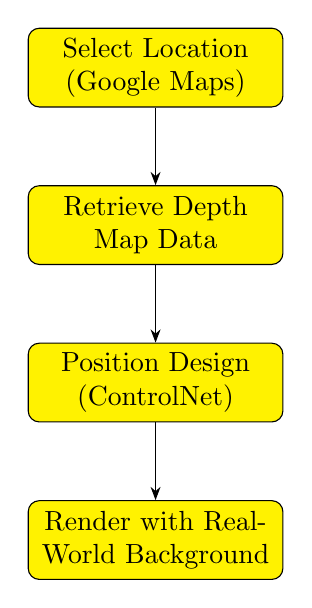
\begin{tikzpicture}[
    node distance=2cm,
    block/.style={rectangle, draw, fill=yellow, rounded corners, minimum width=3cm, minimum height=1cm, text width=3cm, align=center},
    arrow/.style={-Stealth}
  ]

  \node[block] (selectlocation) {Select Location (Google Maps)};
  \node[block, below of=selectlocation] (depthmap) {Retrieve Depth Map Data};
  \node[block, below of=depthmap] (controlnet) {Position Design (ControlNet)};
  \node[block, below of=controlnet] (rendering) {Render with Real-World Background};

  \draw[arrow] (selectlocation) -- (depthmap);
  \draw[arrow] (depthmap) -- (controlnet);
  \draw[arrow] (controlnet) -- (rendering);

\end{tikzpicture}




\subsubsection{Mass \& Volume Calculations}
\begin{itemize}
\item \textbf{Automated Analysis}: Based on the dimensional information from the CAD model and the CMF properties specified in the prompt, the system automatically calculates the estimated weight, volume, and material costs of the design. For example, if the prompt specifies "brushed stainless steel" for a bench frame, the system will calculate the volume of the frame, reference the density of stainless steel, and then calculate the estimated weight and cost based on current market prices.
\item \textbf{Environmental Impact}: The system estimates the environmental impact of the design based on the chosen materials and manufacturing processes. This could involve calculating the carbon footprint based on material extraction, processing, and transportation data. 
\item \textbf{Automated RFQ Generation}: The system can automatically generate requests for quotations (RFQs) based on the calculated material requirements and manufacturing specifications. This could involve automatically filling out web forms or generating emails pre-populated with the relevant design and material information, streamlining the process of obtaining quotes from suppliers.
\end{itemize}

\subsubsection{Design Callouts}
\begin{itemize}
\item \textbf{Automated Callout Generation}: The system can automatically generate professional-style design callouts on the rendered images. These callouts use image segmentation techniques to identify relevant design elements and associate them with text annotations based on the prompt or predefined rules. For example, a prompt like "highlight the ergonomic features" could trigger callouts pointing to the curved backrest, adjustable lumbar support, and padded armrests, with corresponding annotations describing these features. In conjunction with the environmental analysis module previously discussed, callouts with kg/CO2e can then be generated for the drawing to help the design be aware of the potential environmental consequences of their material choices.
\item \textbf{Editable Annotations}: Designers have full control over the generated callouts. They can edit the text, adjust the positioning, change the style, and add or remove callouts as needed. This allows for precise and personalized annotation of the design.
\item \textbf{Searchable PDF Export}: When exporting the rendering as a PDF, the callouts are embedded as searchable text elements, facilitating easy navigation and reference. This ensures that the annotations are not just visual elements but also part of the document's searchable content.
\end{itemize}

\subsubsection{Character Continuity}
\begin{itemize}
\item \textbf{Consistent Character Appearance}: When rendering scenes involving human figures or characters, the system ensures consistent character appearance across multiple variations. This is particularly important when showing a character interacting with the design in different scenarios or using variations to refine the scene's composition.
\item \textbf{Face Swapping}: The system employs face-swapping techniques to maintain a consistent facial appearance for the chosen character, even as other aspects of the scene (e.g., clothing, pose, lighting) vary. This allows the designer to experiment with different variations without needing to re-generate or manually adjust the character's face in each rendering.
\item \textbf{Text-Based Description Matching}: The system analyzes the text prompts for descriptions of the character (e.g., "a woman in her mid-40s with short blonde hair, wearing a business suit"). It uses these descriptions to ensure that the character's appearance consistently matches the designer's intent across different renders, even if the prompt only mentions the character briefly (e.g., "show the woman sitting on the bench").
\end{itemize}

\subsubsection{Dynamic UI Sliders}

This feature provides an advanced level of interactivity and control within the AI-assisted design interface, allowing designers to fine-tune rendering parameters intuitively.

\begin{itemize}
    \item \textbf{Context-Sensitive Sliders}: The interface dynamically generates sliders for controlling rendering parameters based on the context of the text prompt. For instance, if a designer inputs a prompt like "a bench against a backdrop of a stormy sky and waves," the system recognizes elements such as "stormy sky" and "waves." It then generates sliders corresponding to these elements, such as:

    \begin{itemize}
        \item \textbf{Intensity of the Storm}: Adjusts the severity and visual impact of the stormy sky.
        \item \textbf{Turbulence of the Waves}: Controls the roughness or calmness of the water.
        \item \textbf{Brightness of the Lightning}: Modifies the prominence and luminosity of lightning effects.
        \item \textbf{Time of Day}: Alters the overall lighting and atmosphere, from dawn to dusk.
    \end{itemize}

    \item \textbf{Intuitive Control}: These sliders offer a visual and interactive means for designers to adjust parameters without modifying the text prompt directly. This capability allows for:

    \begin{itemize}
        \item \textbf{Granular Exploration}: Designers can incrementally adjust parameters to observe subtle changes in real-time.
        \item \textbf{Rapid Experimentation}: Facilitates quick iteration by enabling immediate visual feedback from slider adjustments.
        \item \textbf{Enhanced Creativity}: Encourages designers to explore a wider range of design variations that they might not have considered through text prompts alone.
    \end{itemize}

    \item \textbf{Parameter Mapping}: The system intelligently maps slider values to the AI model's rendering parameters:

    \begin{itemize}
        \item \textbf{Adaptive Mapping}: Depending on the parameter's complexity, the mapping can be linear, non-linear, or based on a learned function that correlates slider positions with visual outcomes.
        \item \textbf{Real-Time Rendering}: As sliders are adjusted, the AI model updates the rendering in real-time or near-real-time, providing immediate visual feedback.
        \item \textbf{User Customization}: Designers can customize the range and sensitivity of sliders, tailoring the interface to their specific needs and preferences.
    \end{itemize}

    \item \textbf{Integration with Other Features}: The dynamic sliders work in conjunction with other interface elements:

    \begin{itemize}
        \item \textbf{Preset Management}: Slider configurations can be saved as presets for future use or sharing with team members.
        \item \textbf{Modular UI}: Sliders are part of the modular user interface, allowing designers to add or remove them based on the design context.
        \item \textbf{Design Analysis Feedback}: Adjustments made via sliders can be analyzed by the system to provide feedback or suggestions, enhancing the iterative design process.
    \end{itemize}
\end{itemize}

\textbf{Illustrative Example}:

Consider a scenario where a designer is creating a rendering of a modern living room featuring their custom-designed chair. The prompt might be: "A modern living room with large windows overlooking a cityscape, featuring my custom-designed chair in the center."

Based on this prompt, the system generates sliders for:

\begin{itemize}
    \item \textbf{Window Size}: Adjusts the proportion of windows in the scene.
    \item \textbf{Cityscape Lighting}: Controls the brightness and activity level of the city view (e.g., daytime vs. nighttime).
    \item \textbf{Ambient Light}: Modifies the interior lighting to match the desired mood.
    \item \textbf{Chair Material Reflectivity}: Adjusts how reflective the chair's material appears.
\end{itemize}

By adjusting these sliders, the designer can fine-tune the rendering to achieve the exact visual effect they desire, such as transitioning from a bright morning scene to a cozy evening setting without changing the text prompt.




\subsubsection{Patent Drawing Generation}
\begin{itemize}
\item \textbf{Automated Line Art}: The system can automatically generate line art drawings from the CAD model suitable for patent applications. It utilizes edge detection algorithms and vectorization techniques to create clean, precise line drawings that meet the requirements of patent offices (see Figure \ref{fig:automated-design-callout}).
\item \textbf{Annotation Placement}: Annotations such as dimension lines, reference numerals, and technical labels are automatically placed according to patent drawing conventions. The system uses the structured data from the CAD model to accurately determine dimensions and relationships between design elements, ensuring that the annotations are placed correctly and comply with patent regulations.
\item \textbf{Export Format Compliance}: The generated patent drawings are exported in a format compliant with the specific requirements of the target patent office, simplifying the patent filing process.
\end{itemize}


\subsubsection{Design Analysis}
\begin{itemize}
\item \textbf{GPT Integration}: The system integrates with a large language model (LLM) like GPT-3 or a specialized design-focused LLM. This LLM is used to analyze the design in the context of the prompt and identify potential issues or areas for improvement. For example, if the prompt specifies "a park bench made of unfinished hickory wood in West Virginia," the LLM could access external knowledge bases to determine that hickory is susceptible to carpenter ant infestations in that region, flagging a potential durability issue.
\item \textbf{Problem Highlighting}: The LLM analyzes the design for factors like material suitability, structural integrity, ergonomics, and manufacturing feasibility. It flags potential problems and provides feedback to the designer, highlighting areas that might require further consideration or refinement. This feedback can be presented as text-based warnings, visual highlights on the rendered image, or even suggested modifications to the design or materials.
\item \textbf{Contextual Feedback}: The design analysis takes into account the specific context described in the prompt. For example, if the prompt mentions "outdoor furniture," the LLM might check for weather resistance and UV degradation of the chosen materials. The more context the designer provides in the prompt, the more refined and relevant the design analysis feedback will be.
\end{itemize}

\subsubsection{Client Annotation Tools}
\begin{itemize}
\item \textbf{Collaborative Review}: The interface provides tools for clients and reviewers to add annotations, comments, and feedback directly on the rendered images, as illustrated in Figure \ref{fig:modular-ui-texture-style}. This facilitates a more streamlined and collaborative review process, eliminating the need for separate feedback documents or email chains.
\item \textbf{Visual Feedback}: Clients can draw directly on the image, highlight specific areas, add text boxes, or use pre-defined stamps (e.g., "approve," "revise"). This visual feedback is more intuitive and efficient than text-based comments alone, allowing clients to clearly communicate their thoughts and preferences.
\item \textbf{Revision Tracking}: The system tracks all annotations and comments, creating a clear record of the feedback and facilitating iterative revisions. Designers can easily see which areas have received feedback and address specific concerns raised by the client.
\end{itemize}


\subsubsection{Image Security}
\begin{itemize}
\item \textbf{Watermarking}: Invisible watermarks are embedded within generated images to protect the designer's intellectual property. These watermarks can contain information about the designer, the project, or the date of creation and can be used to track the origin of the image if it is distributed without authorization.
\item \textbf{Serialization}: Each rendered image is assigned a unique serial number that can be used to track its usage and distribution. This serial number can be linked to specific client information, allowing the designer to monitor who has access to which images.
\item \textbf{Usage Monitoring}: The system can detect if a watermarked image is used without authorization or if it appears in unauthorized locations online. This monitoring could be automated using image recognition techniques and web crawling tools, providing alerts to the designer if unauthorized use is detected.
\end{itemize}

\subsubsection{Vision Tracking \& Form Review}
\begin{itemize}
\item \textbf{Eye-Tracking Integration}: The system can optionally integrate with eye-tracking technology, using the embedded webcam on a laptop or the rear-facing camera on a mobile phone, for example, to analyze user gaze patterns during the review process.
\item \textbf{Heatmap Visualization}: Eye-tracking data is visualized as heatmaps overlaid on the rendered images for the designer to review. The heatmap can indicate which parts of the design are calling the viewer's attention. The degree to which the viewer's attention aligns with the intended hierarchy of design elements can be quantified, providing valuable insights to the designer. It allows for an objective assessment of whether the viewer is noticing the intended focal points of the design or if their attention is drawn to unintended areas. This feedback can guide the designer in refining the composition, proportions, repetition, and contrast of the design elements to achieve the desired visual impact.
\end{itemize}

\subsubsection{Modular UI}
\begin{itemize}
\item \textbf{Drag-and-Drop Interface}: Designers can drag and drop images or textures onto the design to apply materials or patterns, creating a more intuitive and direct way of customizing the rendering. For example, a designer could drag an image of a specific wood grain onto the bench seat to apply that texture, or drag a color swatch from a palette onto the legs to change their color.
\item \textbf{Texture Blending}: The system supports blending multiple textures together to create more complex and nuanced material effects. For instance, a designer could blend a rough stone texture with a polished metal overlay to create a unique surface finish, allowing for a greater degree of creative control over the material appearance.
\end{itemize}

\subsubsection{Style References}
\begin{itemize}
\item \textbf{Style Transfer}: Designers can apply different artistic styles to renderings by providing reference images. For example, dragging and dropping a still frame from a Pixar movie could instruct the system to render the design in a similar style, even if the prompt describes realistic materials. This allows designers to explore a wide range of aesthetics beyond photorealism.
\item \textbf{Dynamic Style Parameters}: Sliders control the strength and intensity of the applied style. This allows for fine-grained control over the style transfer effect, enabling the designer to blend the reference style with the original rendering to achieve the desired look.
\end{itemize}

\subsubsection{Thematic Sliders}
\begin{itemize}
\item \textbf{Mood and Atmosphere}: Sliders control the overall mood and atmosphere of the rendering. For example, sliders for "brightness," "contrast," "saturation," "warmth," "sharpness," and "depth of field" allow the designer to create a specific emotional tone or visual style without needing to describe these qualities in the text prompt.
\item \textbf{Style Presets}: Thematic sliders can be combined into presets, allowing designers to quickly apply predefined stylistic looks to their renderings (e.g., “cinematic,” “retro,” “minimalist”).
\end{itemize}

\subsubsection{Preset Management}
\begin{itemize}
\item \textbf{Saving and Loading Presets}: Designers can save their preferred rendering configurations as presets, including CMF choices, lighting settings, camera viewpoints, style references, and thematic slider settings. This allows for the reuse of successful rendering styles across different projects or design variations.
\item \textbf{Sharing Presets}: Presets can be shared among team members or publicly, fostering consistency and collaboration in design visualization. This can be particularly useful for maintaining a consistent brand identity or visual style across a design team.
\end{itemize}

\subsubsection{Export Options}
\begin{itemize}
\item \textbf{Image Formats}: The system supports exporting renders in various image formats, including JPG, PNG, TIFF, and EXR, catering to different resolution and quality requirements. This flexibility ensures compatibility with a wide range of design workflows and presentation formats.
\item \textbf{3D Printable Models}: Designers can export the design as a 3D printable model in formats like STL or OBJ, allowing for rapid prototyping and physical evaluation of the design.
\item \textbf{Foldable Paper Models}: The system can generate patterns for creating foldable paper models of the design, providing a tangible and interactive way to explore the form. This can be especially useful in the early stages of design development or for educational purposes.
\item \textbf{Vector Graphics}: Designers can export the rendering as vector graphics (e.g., SVG), enabling scalability and integration with other design software. Vector graphics are particularly useful for creating illustrations, logos, and other design assets that need to be resized without losing quality.
\end{itemize}

\subsubsection{History Tree and Visual Diff}
\begin{itemize}
\item \textbf{Iteration Tracking}: The interface maintains a history of all design iterations, including changes to the prompt, applied materials, lighting settings, and camera viewpoints. This provides a clear record of the design process and allows designers to easily revert to previous versions if needed. This history can be visualized as a tree structure or timeline, providing a clear overview of the design's evolution.
\item \textbf{Visual Diff}: The system highlights the differences between two selected versions of the rendering, visually showing the changes that have been made. This can be implemented by overlaying the two versions and highlighting the areas that have changed, making it easy for the designer to identify the impact of specific modifications. This feature facilitates a clear understanding of the design evolution and aids in iterative refinement.
\end{itemize}

This AI-Assisted Design Interface, with its core rendering functionality and extensive suite of advanced features, empowers designers to leverage the power of AI for creative exploration, efficient workflow, and effective communication. By focusing on natural language interaction, form preservation, and a user-centered design, the interface creates a seamless and intuitive experience that enhances the designer's creative process and unlocks new possibilities in design visualization. The integrated file management, analysis tools, collaborative features, and security measures further streamline the design workflow and address the practical needs of professional designers.

\begin{center}
CLAIMS
\end{center}

A system for generating training data for an AI-assisted design system, comprising:

\begin{itemize}
    \item a CAD interface configured to receive a CAD model having a plurality of objects grouped according to a hierarchical structure;
    
    \item an automated data generation module configured to:
    \begin{itemize}
        \item access the hierarchical structure of the CAD model;
        \item systematically vary visual properties of the objects in the CAD model while maintaining a core design form of the CAD model, thereby generating a plurality of variations of the CAD model;
        \item generate a semantic label for each variation of the CAD model, the semantic label including information about object groupings, applied variations, and design intent;
    \end{itemize}
    
    \item an AI model training module configured to train a text-to-image AI model using the plurality of variations and corresponding semantic labels.
\end{itemize}

The system of claim 1, wherein the visual properties varied by the automated data generation module include at least one of: color, material, finish, texture, camera viewpoint, lighting condition, and background.

The system of claim 1, wherein the automated data generation module varies camera viewpoints using at least one of: hero shot positioning and orbital representation.

The system of claim 1, wherein the AI model training module utilizes Low-Rank Adaptation (LoRA) to fine-tune a pre-trained text-to-image AI model.

The system of claim 1, further comprising an AI-assisted design interface configured to:
\begin{itemize}
    \item receive natural language prompts from a user;
    \item generate renderings of the CAD model based on the natural language prompts and the trained AI model;
    \item allow the user to adjust visual attributes of the CAD model without altering the core design form.
\end{itemize}

The system of claim 5, wherein the AI-assisted design interface further comprises at least one of: automated file management, location-based background integration, cost and environmental impact analysis, automated RFQ generation, design callouts, character continuity management, dynamic UI sliders, patent drawing generation, design analysis feedback, client annotation tools, and image security features.

A method for generating training data for an AI-assisted design system, comprising:
\begin{itemize}
    \item receiving a CAD model having a plurality of objects grouped according to a hierarchical structure;
    \item accessing the hierarchical structure of the CAD model;
    \item systematically varying visual properties of the objects in the CAD model while maintaining a core design form of the CAD model, thereby generating a plurality of variations of the CAD model;
    \item generating a semantic label for each variation of the CAD model, the semantic label including information about object groupings, applied variations, and design intent;
    \item training a text-to-image AI model using the plurality of variations and corresponding semantic labels.
\end{itemize}

\begin{center}
CONCLUSION
\end{center}

This invention significantly advances the field of AI-assisted design by addressing key challenges in training data generation, workflow integration, and designer control. By focusing on form isolation and incorporating a comprehensive suite of advanced features, the system empowers designers to leverage the creative potential of AI while maintaining full control over their design intent and streamlining their workflow. The provided code examples offer a glimpse into the technical implementation of the system, demonstrating how the core functionalities are realized in practice. 

\end{document}